\documentclass[
  utf8,%     More capable input encoding than latin-1.
  parskip,%  For vertical whitespace between paragraphs.  This comes down to more than just using parskip.sty, so it's better to use this class option.
  % S5MP % If you intend to really use margin paragraphs (not recommended!).
%  crop,%     Produce output with crop marks and paper size A4.  Liu-Tryck should like this.  Automatically adds information, including the physical page number, at the top of each page.
       %     Add option 'noInfo' to suppress the info at the top of each page when using option 'crop'.
  % Font options: 'kp' (default), 'times', 'lm'.  The KpFonts (loaded using 'kp'), is the most complete font among the provided options.  Among other, it supports slanted small caps.  See rtthesis.cls for more details regarding the font options.
  largesmallcaps,intlimits,widermath,% Good options to KpFonts.
  sharecounter,nobreak,definition=marks,%  See comments in the results chapter of this document for more information on these options!
  %numbers, % If you want to cite references by numbers, use this option.
  noparts% Use option 'noparts' if you do not make use of part divisions.
]{rtthesis}

\usepackage{mythesis}

% My inclusions/definitions
\def\obs#1{\left<#1\right>}
%\graphicspath{ {images_folder/}{other_folder/}{third_folder/} }
\graphicspath{{figures/}{figures/default/}{figures/created/}{figures/validation}}

\begin{document}
\selectlanguage{english}
\makeFrontPage
\frontmatter
\maketitle
\makeLibraryPage{The \abbrLHC at \abbrCERN is now undergoing an set of upgrades to increase the center of mass energy for the colliding particles to be able to explore new new physical processes. The focus of this thesis lies on the so called phase II upgrade which will preliminarily be completed in 2023. After this upgrade the \abbrLHC will be able to accelerate proton beams to such velocity that each proton has a center of mass energy of 14 TeV.

One disadvantage of this is that it will be harder for the \abbrATLAS detector to isolate unique particle collisions since more and more collisions will occur simultaneously, so called pile-up. 

For 14 TeV there does not exist a full simulation of the \abbrATLAS detector. This thesis instead uses simulated data for the particle collisions and then uses so called smearing functions to emulate the detector responses. 

This thesis focuses on how a mono-jet analysis looking for different \abbrWIMP models of dark matter will be affected by this increase in pile-up rate.

The models which are in focus are thoes which try to explain dark matter without adding new theories to the standard model or \abbrQFT , such as the effective theory D5 operator and light vector mediator models.

The exclusion limits set for the D5 operators mass suppression scale at 14 TeV and 1000 fb$^{-1}$ are 2-3 times better than previous results at 8 TeV and 10 fb$^{-1}$. 

For the first time limits have been set on which mediator masses can be excluded for vector mediator models at 14 TeV.}



%\begin{abstract}[swedish]
 % Det här som vi har hållit på med är jätteviktigt faktiskt och det vi gjort blev bara sååå bra.  Kanske inte helt otippat, men det glass är sååå gott!

Förresten har vi blivit bäst på att skriva rapporter, så nu ska ska vi inte gå in närmare på några detaljer såhär i sammanfattningen.

%\end{abstract}
\begin{abstract}[english]
  The \abbrLHC at \abbrCERN is now undergoing an set of upgrades to increase the center of mass energy for the colliding particles to be able to explore new new physical processes. The focus of this thesis lies on the so called phase II upgrade which will preliminarily be completed in 2023. After this upgrade the \abbrLHC will be able to accelerate proton beams to such velocity that each proton has a center of mass energy of 14 TeV.

One disadvantage of this is that it will be harder for the \abbrATLAS detector to isolate unique particle collisions since more and more collisions will occur simultaneously, so called pile-up. 

For 14 TeV there does not exist a full simulation of the \abbrATLAS detector. This thesis instead uses simulated data for the particle collisions and then uses so called smearing functions to emulate the detector responses. 

This thesis focuses on how a mono-jet analysis looking for different \abbrWIMP models of dark matter will be affected by this increase in pile-up rate.

The models which are in focus are thoes which try to explain dark matter without adding new theories to the standard model or \abbrQFT , such as the effective theory D5 operator and light vector mediator models.

The exclusion limits set for the D5 operators mass suppression scale at 14 TeV and 1000 fb$^{-1}$ are 2-3 times better than previous results at 8 TeV and 10 fb$^{-1}$. 

For the first time limits have been set on which mediator masses can be excluded for vector mediator models at 14 TeV.
\end{abstract}
\begin{acknowledgments}
I wish to dedicate this thesis to my mathematics teacher Ulf Rydmark without whom I would not have studied physics.

A big thank you to my family, fiancée and friends who have supported me throughout my education. A warm thank you to my friend Joakim Skoog who altered some of the images for me.


I want to thank my supervisor Christophe Clément and all those who helped me at Stockholm University. \\
I also want to thank my examiner Magnus Johansson, who always took time to answer any question from and support his students. \\ 
A special thank you to Professor Irina Yakimenko without whom my master years would have been duller and probably impossible.\\
Finally I want to thank someone someone for proofreading my

  \addvspace{1em}
  \begin{flushright}
    \textit{%
      Linköping, May 2014\\
      Sven-Patrik Hallsjö%
    }
  \end{flushright}
\end{acknowledgments}

\tableofcontents
%\newpage
% Add a list of all figure captions and makes sure that the tile is set to the right as the rest of them.
%\begin{flushright}
%\listoffigures
%\end{flushright}
\begin{notation}% Passing the option "old" to the notation environment will redefine the notationtabular environment so that it produces an old style LaTeX tabular instead of a ctable.sty style tabular.
  \centering

  \begin{notationtabular}{Notations}{Notation}{Explanation}
  barn(b) & 1 barn(b)$=10^{-24}$ cm$^2$ \\
  $\oplus$ & $a\oplus b = \sqrt{a^2 + b^2}$, $a\oplus b\oplus c = \sqrt{a^2+b^2+c^2}$ \\
    %$\naturals$ & Mängden av naturliga tal \\
   \end{notationtabular}

  \begin{notationtabular}{Abbreviations}{Abbreviation}{Expansion}
  
\abbrATLAS\index{ATLAS@\abbrATLAS!abbreviation} & A large Toroidal LHC ApparatuS \\
\abbrCERN\index{CERN@\abbrCERN!abbreviation} & Organisation européenne pour la recherche nucléaire\footnotemark \\
\abbrCMS\index{CMS@\abbrCMS!abbreviation} & Compact Muon Solenoid\\
\abbrCR\index{CR@\abbrCMS!abbreviation} & Control Region\\
\abbrLHC\index{LHC@\abbrLHC!abbreviation} & Large Hadron Collider \\
\abbrMC\index{MC@\abbrMC!abbreviation} & Monte Carlo \\
\abbrRMS\index{RMS@\abbrRMS!abbreviation} & Root Mean Square \\
\abbrSM\index{SM@\abbrSM!abbreviation} & the Standard Model of particle physics \\
\abbrSR\index{SR@\abbrSM!abbreviation} & Signal Region \\
\abbrWIMP\index{WIMP@\abbrWIMPS!abbreviation} & Weakly Interacting Massive Particle \\
\abbrWIMPS\index{WIMPS@\abbrWIMPS!abbreviation} & Weakly Interacting Massive ParticleS \\
\abbrQED\index{QED@\abbrQED!abbreviation} & Quantum ElectroDynamics \\
\abbrQFT\index{QFT@\abbrQFT!abbreviation} & Quantum Field Theory \\
\abbrQM\index{QM@\abbrQM!abbreviation} & Quantum Mechanics \\
  \end{notationtabular}
 
 \footnotetext{Originally, Conseil Européen pour la Recherche Nucléaire}
\end{notation}


\mainmatter
\chapter{Introduction}\label{cha:intro}
Discrepancies in measurements of the rotations of galaxies indicate the presence of a large amount of matter which interacts through gravity, though not electromagnetically making it invisible to our telescopes. This matter is commonly referred to as dark matter. Since no known or hypothesised particle in the standard model of particle physics can be used as a candidate for dark matter, this has opened the door for new physics. Aside from dark matter there are other phenomena, such as the neutrino mass and the hierarchy problem, that can not be explained today. One of the proposed models to correct these discrepancies is known as Supersymmetry (\abbrSUSY).  

At the Organisation européene pour la recherche nucléaire (\abbrCERN) the interest now lies to discover any evidence of \abbrSUSY. Among other searches one is fixed at looking for so called weakly interacting massive particles (\abbrWIMPS) which may be a candidate for dark matter. It is usually impossible to detect any interaction of dark matter candidates on the subatomic scale, however through looking at proposed interactions, searching for assumed decay channels and inconsistencies in momentum conservation it is hoped that signs will be found. Though as of \today\ none have been found. 

Both these experiments and current theories now show that higher energies are required at the \abbrLHC to be able to see any signs. This is why the \abbrLHC and all detectors are undergoing a vast upgrading program \citep{ATLAS:LOI2}.
In this thesis focus will be on the last part of the upgrade due for completion in 2023, known as the high luminosity-\abbrLHC phase II upgrade; and also on the \abbrATLAS detector.

In this chapter an introduction to both the theoretical and experimental details required to understand the method and results is given. 

\newpage
\section{Research goals}\label{sec:goals}
This research took place at Stockholm University from January 7th until \textbf{when?}
During the research period the following tasks were set up and performed/answered:
\begin{itemize}
\item Implement a C++ programme that loops over the collisions inside the signal and background datasets.	
\item For each collision retrieve the relevant observables (variables used to	 extract the signal over the background) and apply "smearing functions" to emulate the effect of the high luminosity on the observables. 	
\item For both signal and background datasets, compare observables before and after smearing. What observables are the least/most affected?	
\item Implement selection criteria that selects the signal collisions efficiently while reduces significantly the background. In a first step the selection criteria should be taken from existing studies.
\item Selection criteria can be evaluated and compared with each other using a figure of merit P, that measures the sensitivity of the experiment to the	 dark matter signal. Calculate P for the given selection criteria before and after smearing.
\item What is the effect of the high luminosity (smearing) on the value of P?
\item Investigate other selection criteria and observables, to mitigate the effect of high luminosity. Use P to rank different criteria after smearing.
\item Conclude on the effect of the high luminosity on the sensitivity for dark matter and possible ways to mitigate its effects using alternative observables and selection criteria. 
\end{itemize}
\newpage
\section{Theoretical Background}\label{sec:tb}
The following is a short description of the theory which is required to understand this thesis. 
\subsection{Quantum mechanics and quantum field theory}\label{sec:tb:subsec:qm}
In the beginning of the 20th century, some physical phenomena could not be explained by classical physics, for example the ultra-violet disaster of any classical model of of black-body radiation, and the photoelectric effect.\citep{Bransden:2000}
It was these phenomena that led to the formulation of quantum mechanics (\abbrQM), where energy transfer is quantized and particles can act as both waves and particles at the same time. \citep{Hallsjo:2013}

Combining \abbrQM with classical electromagnetism proved harder than expected, colliding a photon(em-field) and an electron (particle/wave) is quite tricky. (Refer to scattering) One idea that came from this was to explain them both in the same framework, field theory.
Also, trying to incorporate special relativity into \abbrQM suggested a field description. (Metric description and bending of gravitational fields).
The culmination of both of these problems is Quantum electrodynamics (\abbrQED)which with incredible precision explains electromagnetic phenomena including effects from special relativity.\citep{Zee:2003}


Something something Lagrangian of these processes something something can be simply viewed through Feynman diagrams.
Explain four-vectors quickly.
Somehow end up with Feynman diagrams.

Also mention special rel + qm expects and now proven antimatter.

Speak about: Why \abbrQM, Lagrangian refer to classical mechanics, end with hand of to particle physics. need to explain observables.
Theoretical Particle physics comes from Feynman diagrams!

Dont forget to explain cross-sections from qft.

Find more information in \citep{Goldstein:2001,Bransden:2000, Zee:2003}.

\subsection{Nuclear, particle and subatomic particle physics}
Can be seen as the experimental counterpart to quantum mechanics.
Many could argue that these branches started after Ernest Rutherford famous gold foil experiment (reference), where he discovered that matter is composed of matter with a nucleus, a lot of empty space and electrons. This and more sparked the curiosity to see what the nucleus was made of and so on... 

The discovery of the quark dividing of bosons/fermions different generations. Fundamental particles. Basically all of 20th century physics. 

Something so that a description of particles are in here, end with standard model.
Content should be enough for the rest of the thesis regarding collisions etc.
Luminosity!

\textbf{Explain hadrons...}

From \citep{Burchan:1995}

\subsection{The standard model of particle physics} 
The standard model of particle physics, simply the standard model (\abbrSM).
How and why is there a standard model? give the Lagrangian and refer to all the different interactions that are included. Which then combines \abbrQM with subatomic particle physics.

 From \citep{Burchan:1995} and more for the problems?
 
Mention Antimatter!
Is it proved? What problems exist? 
\begin{itemize}
\item No QFT for general relativity! Thus there is no link between gravity and the SM.
\item Experimentally it has been shown that neutrinos have mass, though in SM they do not!
\item Asymmetry between matter and antimatter can not fully be described.
\item No dark matter candidate!
\item Dark energy?
\end{itemize} 
\subsection{Dark matter}\label{sec:dark}
A very quick introduction was given in the beginning of this chapter. Dark matter is the name given to the solution to the discrepancies of galactic rotations. 
\textbf{Check the email regarding half-time meeting} Image etc.

After this the big question arises, what could this dark matter consist of? One possible explanation comes from \abbrSUSY where there exists particles that are massive though will not interact electromagnetically.

Dark since no electromagnetic interaction, matter since gravitational interaction. Mention that the interest is cold dark matter, thus massive [GeV] scale.

There are several theories how to detect dark matter in proton-proton collisions such that occur at \abbrCERN \textbf{Refer to section?}. 
\begin{itemize}
\item Ordinary matter interacting with ordinary matter can produce dark matter, known as production.
\item Dark matter interacting with ordinary matter can produce dark matter, known as direct detection.
\item Dark matter interacting with dark matter can produce ordinary matter, known as indirect detection.
\end{itemize} 
In this theses the focus lies with production.
\subsection{Beyond the standard model: Supersymmetry}
In the early 1970:s similar as \abbrQED expansion with antimatter due to (integral which one diverged?). Similarly to this, an expansion with a similar symmetry having bosons instead of fermions and the reverse. These symmetrical particles are known as supersymmetrical partners. The \abbrSUSY partner of a boson is denoted as sfermion (squarks and sleptons) whereas the \abbrSUSY partner of a fermion is denoted as bosinos (gauginos).  \textbf{Image used by Sara particles with their equivalents.}

Different problems, hierarchy, etc

Bring up different expansions. Here I will talk about supersymmetry (\abbrSUSY) end with neutrilino
Explain how we get wimps:
Weakly interacting massive particles (\abbrWIMPS) are a candidate to explain Dark matter, it is this candidate which is considered in this thesis. Where these 
\abbrWIMPS. 
Minimal Supersymmetric Standard Model

Supersymmetry: Every boson has a supersymmetrical fermion, and the reverse.

Some from, else from licentiates \citep{Martin:1998,Dine:1981,Pavel:2014}

\subsection{Effective field theory}
In quantum field theory the objective is usually to find the part of the Lagrangian which explains a type of interaction, known as the operator of the interaction and also to find the probability amplitude (cross-section) for a certain interaction. For complicated processes it is easier to employ certain conditions so that the small scale phenomena are simplified and the whole picture understood. This called using an effective field theory and the idea can be in \figureref{fig:feymanc}. The operator can be found through assuming the possible interactions and using the effective field theory \citep{Zee:2003}. The cross-sections can be found through the Feynman diagrams as described in \subsectionref{sec:tb:subsec:qm}. 
%trim=left botm right top.
 % good for finding limits \fbox{\includegraphics[scale=•]{•}}
 \begin{figure}[!ht]
    \subfloat[Electromagnetic interaction.\label{fig:feymanc:a}]{%
     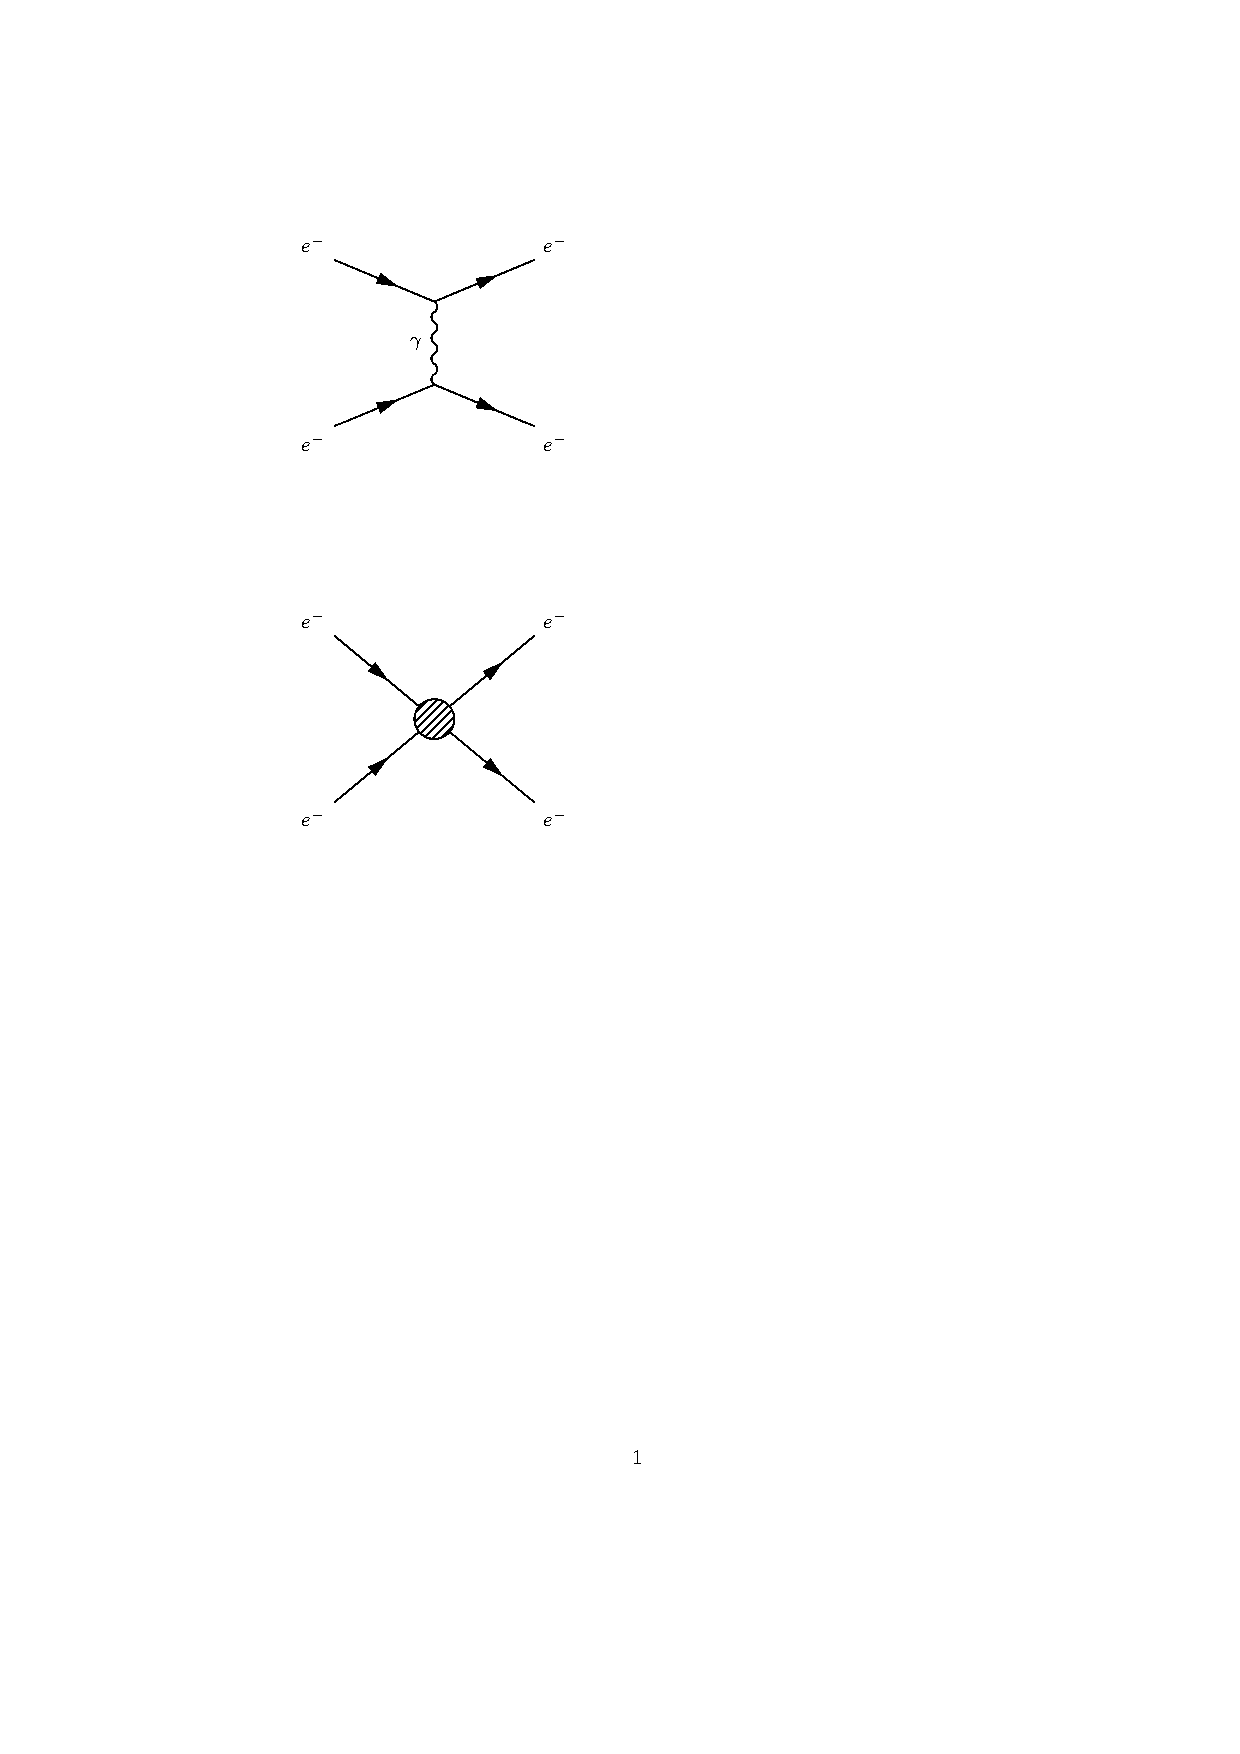
\includegraphics[trim=5cm 22cm 11cm 4cm,clip=true, width=0.5\textwidth]{myfeynman.pdf}
    }
    \hfill
    \subfloat[Effective diagram of \figureref{fig:feymanc:a}.\label{fig:feymanc:b}]{%
      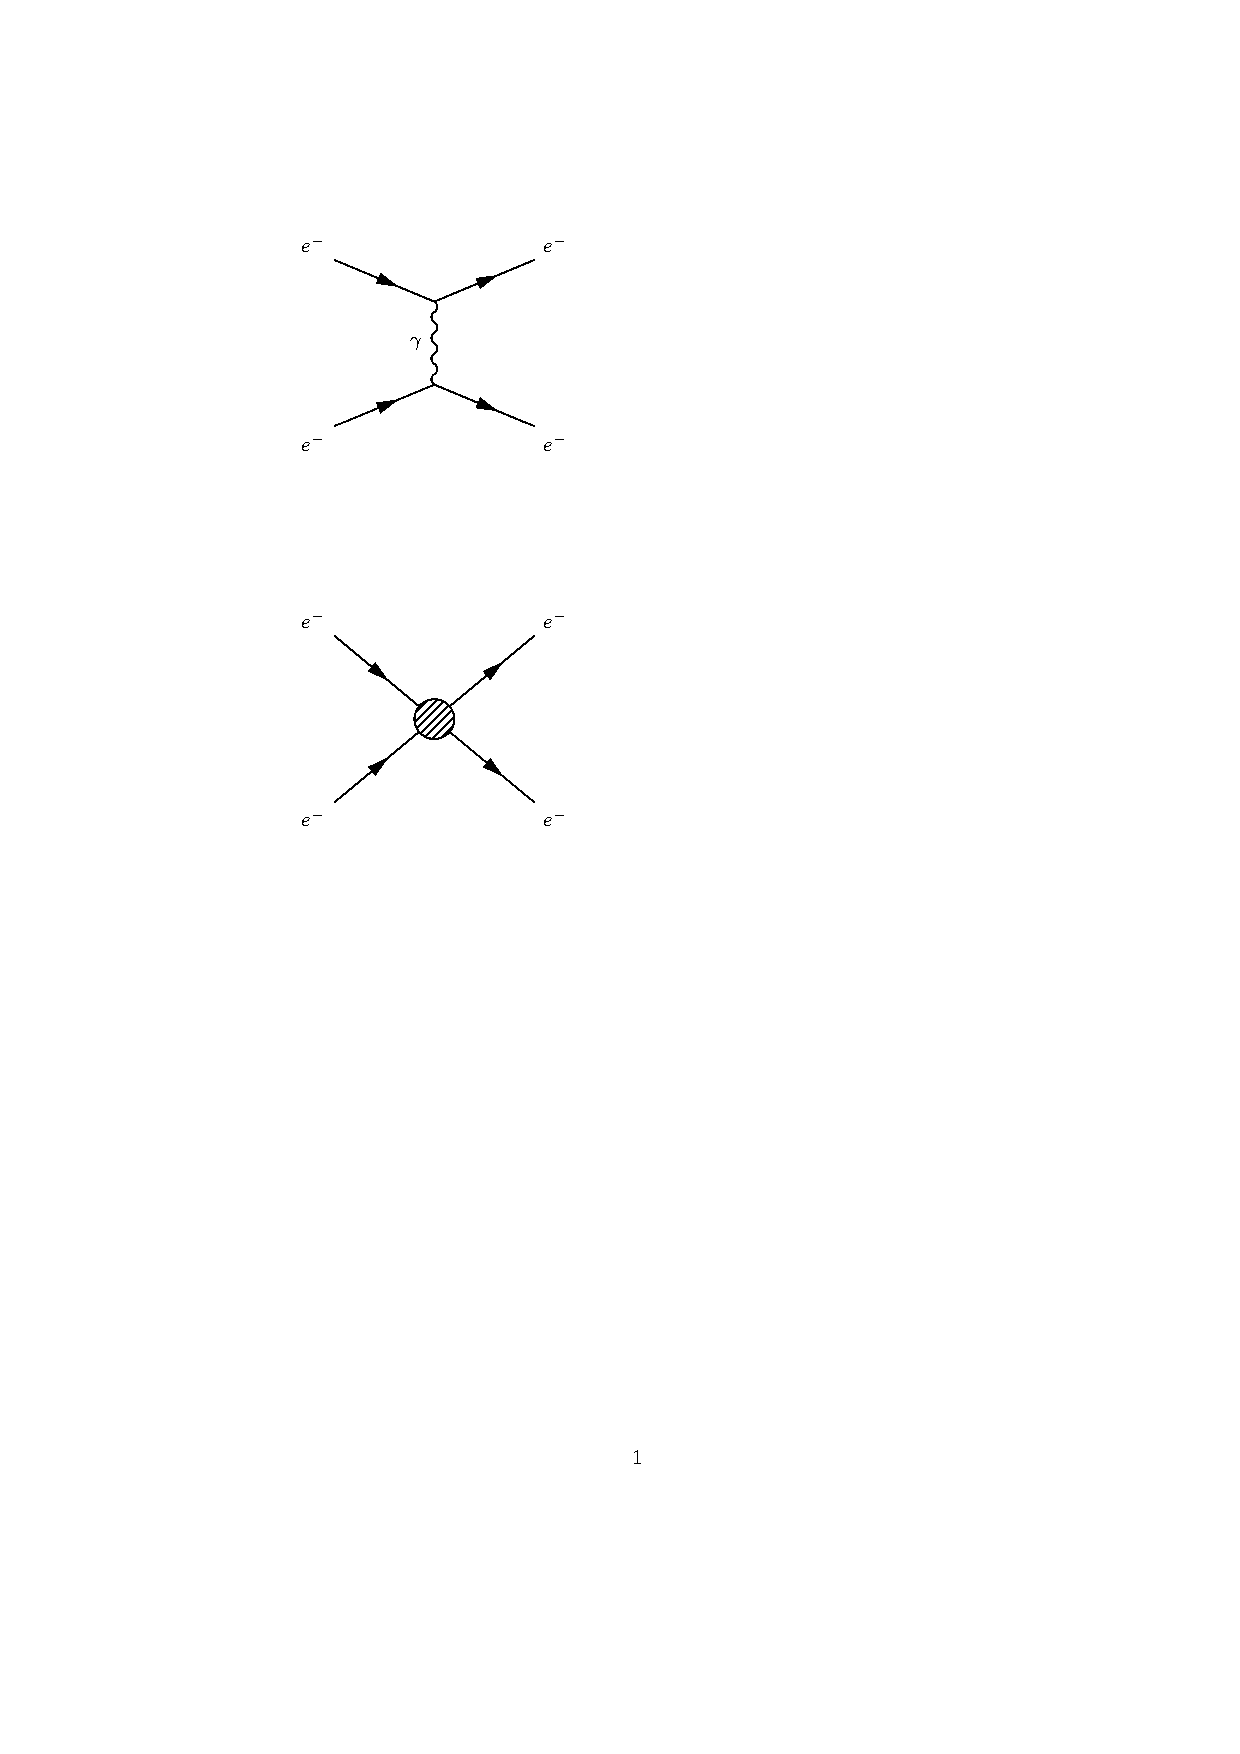
\includegraphics[trim=5cm 15.7cm 11cm 10.3cm,clip=true, width=0.5\textwidth]{myfeynman.pdf}
    }
    \caption{Feyman diagram of an electron-electron scattering, both as an ordinary diagram and as its effective version, where the details are hidden in the blob.}
    \label{fig:feymanc}
  \end{figure}

In this thesis the same effective field theory as in \citep{82.116010,Goodman:2010} will be considered. The \abbrWIMP (usually denoted $\chi$) is assumed as the only particle in addition to the standard model fields. $\chi$ will be assumed odd under some $Z_2$ symmetry. This means that an even number of $\chi$ must be in every coupling. It is assumed that the whatever mediator exists is heavier that the \abbrWIMPS, meaning that their interactions are in higher order terms of the effective field theory and thus not included in the operators. For simplicity, the \abbrWIMPS are assumed to be \abbrSM singlets, thus invariant under \abbrSM gauge transformations, and the coupling to the Higgs boson is neglected.

The focus for the operators will be quark bilinear operators on the form $\bar{q}\Gamma q$ where $\Gamma$ is a 4 $\times$ 4 matrix of the complete set, 
\begin{equation}
\Gamma = \left\lbrace 1,\gamma ^5,\gamma ^\mu,\gamma ^\mu \gamma ^5, \sigma ^{\mu \nu} \right\rbrace
\end{equation}
This will dictate how the operators are written, more of why this is done can be found in \citep{82.116010,Goodman:2010,Zee:2003}.

This, together with the \textbf{couplings to GG} define an effective field theory of the interaction of singlet \abbrWIMPS with hadronic matter. It is a non-renormalizable field theory which will break down when the mediator mass is close to the mass of the \abbrWIMP .
The condition for this is derived in \citep{82.116010} and gives:
\begin{equation}
M > 2 m_\chi
\end{equation}
where $m_\chi$ is the mass of the \abbrWIMP and M is the mass of the mediator. There is also the requirement that:
\begin{equation}
M \lesssim 4 \pi M_*
\end{equation}
where $M_*$ is the energy scale where the effective theory is no longer a good approximation.

In this work, WIMPS are assumed to be Dirac fermions (half integer spin and is not its own antiparticle). 
 
In \tableref{tab:operators} the operators which are integrated out via the effective field theory and are of interest in this thesis are given.
\renewcommand{\arraystretch}{1.5} %Change height of tabel
\begin{table}[H]
\begin{center}
    \begin{tabular}{ | l | l | l | l |}
    \hline
    Name & Initial state & Type & Operator \\ \hline
  	D1 & qq & scalar & $\frac{m_q}{M^3_*} \bar{\chi} \chi \bar{q} q$ \\ \hline
  	D5 & qq & vector & $\frac{1}{M^2_*} \bar{\chi} \gamma^\mu \chi \bar{q} \gamma_\mu q$ \\ \hline
  	D8 & qq & axial-vector & $\frac{1}{M^2_*}\bar{\chi}\gamma^\mu \gamma^5 \chi \bar{q} \gamma_\mu \gamma^5 q $ \\ \hline
  	D9 & qq & tensor & $\frac{1}{M^2_*} \bar{\chi}\sigma^{\mu \nu} \chi \bar{q} \sigma_{\mu \nu} q  $\\ \hline
  	D11 & gg & scalar & $\frac{1}{4M^3_*}\bar{\chi}\chi \alpha_s (G^a_{\mu \nu})^2 $\\ \hline
  	\end{tabular}

  	\caption{From \citep{CERN-PH-EP-2012-210}}
  	\label{tab:operators}
  	  	\end{center}
    \end{table}
\renewcommand{\arraystretch}{1.0}  %Back to default
Where D denotes that the \abbrWIMPS are assumed to be Dirac fermions.

\textbf{Also what is looked at is light vector-mediators similar to Z!}

\subsection{Search for \abbrWIMPS}
The search of \abbrWIMPS is based on a mono-jet analysis which is described in \subsectionref{sec:experiment:subsec:monojet}. 

Since the search for \abbrWIMPS at the \abbrLHC is based on looking at $E_T^{Miss}$ it will be canonical though the experiment can no establish if a \abbrWIMP is stable on a cosmological time scale and thus if it is a Dark matter candidate \citep{CERN-PH-EP-2012-210}

Include SUSY-feynman?

What is it? Why at \abbrCERN/\abbrATLAS? Candidates?
Dark matter is something which does not interact electromagnetically however it does have a gravitational effect on nearby bodies.
Cold dark matter?
Non-barionic dark matter. Why not barionic?
\abbrWIMPS, wimps as candidates.
How is this detectable at \abbrATLAS? Finish with this. Refer next chapter and that neutralinos are a candidate.

\newpage
\section{Experimental overview}\label{sec:experiment}
What was used in this research and what needs to be explained? Upgrade, pileup etc.
Somewhere here explain how the radial coordinate system is defined.
\subsection{\abbrLHC}
The Large hadron collider (\abbrLHC) is a particle accelerator located at \abbrCERN near Geneva in Switzerland, see \figureref{fig:lhc}. The accelerator was built to explore physics beyond the standard model and to make more accurate measurements of standard model physics. Before it was shut down for an upgrade in 2012 it was able to accelerate two proton beams to such a velocity that they had an energy of 4 TeV which gives a center of mass energy, $\sqrt{s}=8$ TeV. It should be noted that the proton beam is not homogeneous, it is comprised of bunches of protons with enough spacing that bunch collisions can happen independent of each other.Apart from the energy, the ability for an accelerator to produce interactions can be calculated through the instantaneous luminosity of the \abbrLHC was $10^{34}$ cm$^{-2}$s$^{-1}$ or $10$nb$^{-1}$s$^{-1}$ where 1 barn(b)$=10^{-24}$ cm$^2$. All values taken from \citep{lumires}.
\begin{figure}[H]
\begin{center}
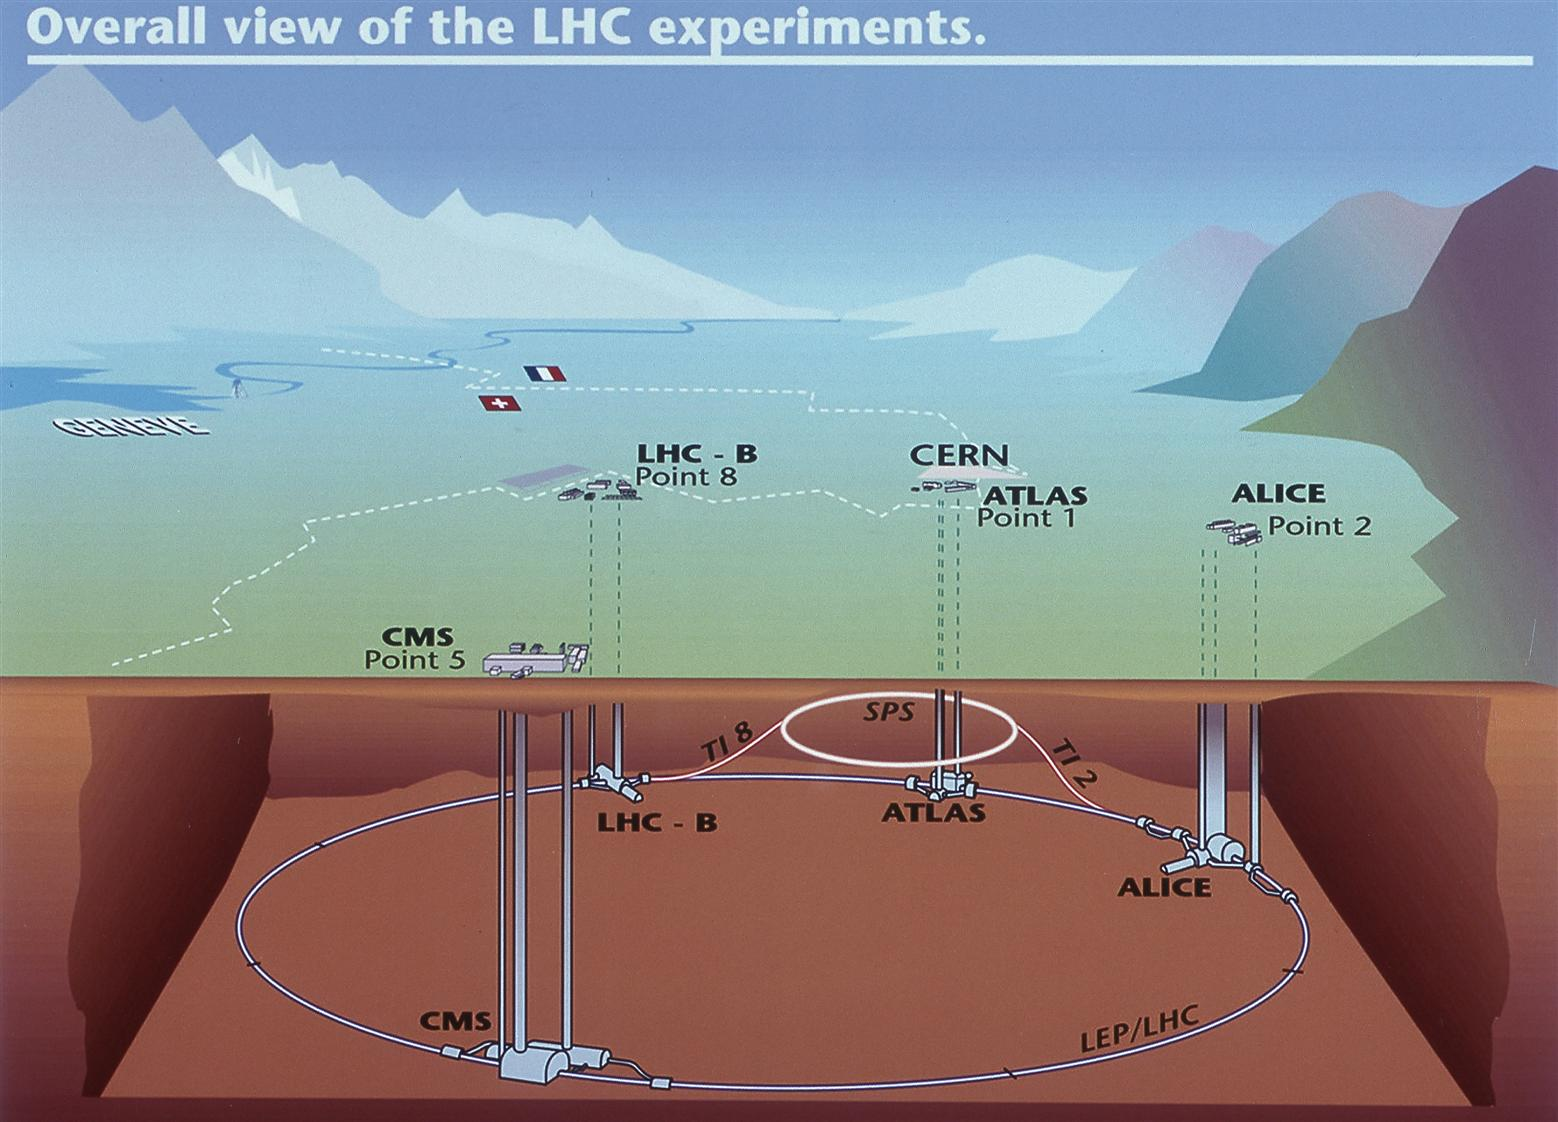
\includegraphics[width=\linewidth]{lhc.jpeg}
\caption{Figure showing the \abbrLHC and the different detector sites\citep{lhcimage}}
\label{fig:lhc}
\end{center}
\end{figure}
The instantaneous luminosity can be defined in different ways depending on how the collision takes place. For two collinear intersecting particle beams it is defined as:
\begin{equation}
\mathscr{L} = \frac{fkN_1 N_2}{4\pi \sigma_x \sigma_y}
\end{equation}
where $N_i$ are the number of particles in each of the bunches, f is the frequency at which the bunches collide , k the number of colliding bunches in each beam, and $\sigma_x$ ($\sigma_y$) is the horizontal (vertical) beam size at the interaction point. Since the instantaneous luminosity increases quadratically with more particles in each bunch this would be a good strategy. However aside from the difficulties to create and maintain a beam with more particles, a large $N_i$ increases the probability for multiple collisions per bunch crossing, referred to as pile-up. Pile up will be a key aspect which is described more in \subsectionref{sec:experiment:subsec:pileup}. 

The expected number of events can be calculated by using the instantaneous luminosity through the following:
\begin{equation}
N=\sigma \int \mathscr{L} dt := \sigma \Lagr
\end{equation}
where $\Lagr$ is the luminosity and $\sigma$ is the cross section which is often measured in barn.
The luminosity is a measurement of total number of interactions that have occurred over time. Before the \abbrLHC was shut down this values was 20.8 fb$^{-1}$.

The cross section is defined through the integral of the differential cross section, as explained in \subsectionref{sec:tb:subsec:qm}, over the whole solid angle:
\begin{equation}
\sigma = \oint d\Omega \frac{d\sigma}{d\Omega}
\end{equation}
The cross section is therefore a measure of the effective surface area seen by the impinging particles, and as such is expressed in units of area. The cross section is proportional to the probability that an interaction will occur. It also provides a measure of the strength of the interaction between the scattered particle and the scattering center.
Further details can be found in reference~\citep{Herr:2006}

\subsection{\abbrATLAS}
As seen in \figureref{fig:lhc}, there are several detectors at \abbrCERN. One of these is a large toroidal \abbrLHC apparatus (\abbrATLAS) which is a general purpose detector that uses a toroid magnet. Its goal is to observe several different production and decay channels. The detector is composed of three concentric subdetectors, the Inner detector, the Calorimeters and the Muon spectrometer.

Most and more in \citep{1129811}
\subsection{Coordinate system}
The coordinate system of ATLAS, seen in \figureref{fig:coordinatesystem} is a right-handed coordinate system with the x-axis pointing towards the centre of the LHC tunnel, and the z-axis along the tunnel/beam (counter clockwise) seen from above. The y-axis points upward.
The origin is define as the interaction point.
A cylindrical coordinate system is also used for the transversal plane. (R,$\phi$,Z).
For simplicity the pseudorapidity of particles from the primary vertex is defined as:
\begin{equation}
\eta = - \ln( \tan\frac{\theta}{2})
\end{equation}
where $\theta$ is the polar angle (xz-plane) of the particle direction measured from the positive z-axis. 
$\eta$ is through this definition invariant under boosts in the z-direction.

It is quite common to calculate the distance between particles and jets in the $(\eta,\phi$) plane, $d=\sqrt{\Delta \eta + \Delta \phi}$  

\begin{figure}[ht]
\begin{center}
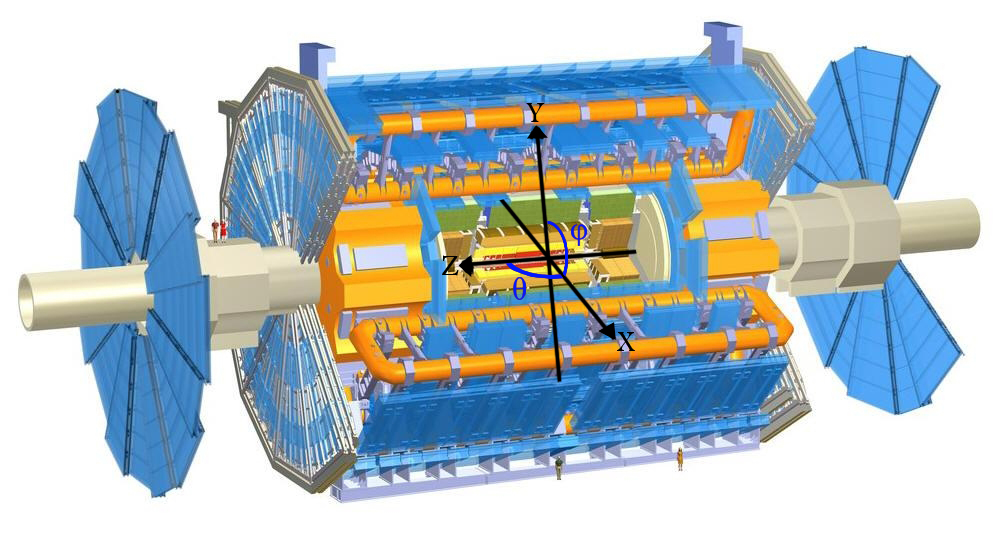
\includegraphics[width=\linewidth]{particle_collider.jpg}
\caption{Figure showing the \abbrATLAS detector and the definition of the orthogonal Cartesian coordinate system. Image altered from\citep{coordimage}}
\label{fig:coordinatesystem}
\end{center}
\end{figure}

\subsection{Calorimeter}
\subsection{Reconstructing data}
Give a general description.

In this thesis, truth = Montecarlo. 
Reconstructed data = that which is seen in the detectors, which is the smeared data.
\subsection{Pile-up}\label{sec:experiment:subsec:pileup}
\subsection{Mono-jet analysis}\label{sec:experiment:subsec:monojet}
What is a jet? why are we only looking at transverse missing energy? 

\subsection{Phase II high luminosity upgrade}
Talk about the upgrade schedule. \citep{ATLAS:LOI2}
I am looking at the upgrade which will be done at \abbrCERN and will be completed around 2022-2023 and is denoted High Luminosity-\abbrLHC Phase 2 upgrade. When this is running the following is expected:
\renewcommand{\arraystretch}{1.5} %Change height of tabel
\begin{table}[H]
\begin{center}
    \begin{tabular}{ | l | l | l |}
    \hline
    Entity & Expected & Last run (2012) \\ \hline
  	Luminosity & 1000-3000 fb$^{-1}$ & 20.8 fb$^{-1}$ \\ \hline
  	Pile-up & $\obs{\mu}=200$ & $\obs{\mu}=20.7$ \\ \hline
  	Center of mass energy & $\sqrt{s}=14$ TeV &  $\sqrt{s}=8$ TeV \\ \hline
  	\end{tabular}
  	
  	\caption{Expected running values for the Phase II HL-upgraded \abbrLHC with older values for comparison. REFERENCE?}
  	\label{tab:expectvalues}
  	\end{center}
    \end{table}
    \renewcommand{\arraystretch}{1.0}  %Back to default
Taken from "a short explanation of different terminology by me" Find a cern source.
Assumed effects, timespan when will it be done?

\section{Monte Carlo simulation, truth data}
What it is in short detail. How it is set-up and what it produces for us in this context. 
Where does it come from? Perhaps quick explanation of different programs?
\section{ROOT}
A wonderful tool for processing data by programming in C++ and so on... Reference to root homepage?
\chapter{Method}\label{cha:meth}
In this chapter the methodology used to perform the tasks given above in \sectionref{sec:goals}.
\newpage
\section{Validation of smearing functions} 


Find more information in my presentation. also mention no pile-up dependence of leptons.
For the proposed upgrade of the LHC.

The validation was done for \textbf{what MCdata? and validated for which pile-up?}

\subsection{Smearing}
One might assume that using a Monte Carlo simulation it would be easy to model and simulate the whole process, from collision to detection and reconstruction in the upgraded LHC. It is possible, but it requires a lot of computing power. Instead one can use one simulation and a mathematical model to calculate the estimated response in the detector. This was validated and used in this thesis to be able to create the data needed for further analysis. 

This was done by using a Monte Carlo simulation of a proton-proton collision the applying official Truth to reco code that was developed using previous studies \citep{ATL-PHYS-PUB-2013-004}; to simulate the effect that pile-up would have on the signals that come from the detectors and the reconstruction of these.

The code uses the experimental data from the previous studies to smear the reconstructed energy and momenta; It does not however alter the direction of the momenta. Other experimental data was used and shows that only jets and $E^{miss}_T$ are affected by pile-up. 

The data was taken from these processes:
\begin{itemize}
\item Electron, W$\rightarrow e\nu$
\item Muon, W$\rightarrow \mu \nu$
\item $\gamma$, $\gamma$ + Jet sample.
\item Tau, W$\rightarrow \tau \nu$
\item Jets, Jet sample.
\item $E_T^{Miss}$, Z$\rightarrow \nu \nu$ + Jet sample
\end{itemize}

That this is true can be shown from \textbf{figures and references from nonpileupdep.txt presentation!}. The smearing functions should be given!

Perhaps under results?
\subsection{Validation}
To validate the smearing code comparisons were made with \citep{ATL-PHYS-PUB-2013-004}. 

Parametrization used according to the paper \citep{ATL-PHYS-PUB-2013-004}. What results and what did I get/say in my presentation? Use that in results Perhaps even write something better than the original that can be used to explain this again.

\begin{itemize}
\item For electron, photon:\\
$\sigma=0.3\oplus 0.1\sqrt{E(GeV)}\oplus 0.01E(GeV)$, $|\eta|<$ 1.4, \\
$\sigma=0.3\oplus 0.15\sqrt{E(GeV)}\oplus 0.015E(GeV)$, 1.4 $<|\eta|<$ 2.47 
\item For muon: $\sigma=\frac{\sigma_{id} \sigma_{ms}}{\sigma_{id} \oplus \sigma_{ms}}$\\
$\sigma_{id}=P_T(a_1 \oplus a_2 P_T)$, $\sigma_{ms}=P_T(\frac{b_0}{P_T} \oplus b_1 \oplus b_2 P_T)$
\item For tau: $\sigma =(0.03\oplus \frac{0.76}{\sqrt{E(GeV)}})E(GeV)$, for 3 prong. 
\item For Jet: $\sigma = P_T(GeV)(\frac{N}{P_T} \oplus \frac{S}{\sqrt{P_T}} \oplus C)$ \\
Where N, S, and C are parameters found in the paper, that depend on $\eta$. 
\\N is also dependent on the pile-up that is simulated.
\item For $E_T^{miss}$: $\sigma = (0.4+0.09\sqrt{\mu})\sqrt{\sum E(GeV)+20\mu}$
\end{itemize}
Here each sigma represents the \textbf{absolute?} rms.

\textbf{One prong for tau exists, though was not used!}

Remember for the discussion to mention different types of rms, relative or absolute. and the problem which occurred with this and the papers faults.

\section{Evaluating dark matter signals}
The main goal of the thesis is to investigate if certain dark matter signals can be detected after the high luminosity upgrade. One immediate worry is that the background will be large in comparison to the signal, thus making it undetectable. 

The following signals models have been used:
\textbf{Here only the operators should be explained, or different models. The names and the MC here or in appendix?} They are explained somewhat in the introduction.
Each of these has been evaluated in different signal regions and the detectability has been evaluated using a statistical P-value. This process has been performed at different pile-up values. 

\textbf{What background existed? How was it simulated in MC? Should that be here or in appendix?}


\subsection{Signal to background ratio}
What I am doing now, looking at what signal? What are the different background processes? What and why was the weight used?

Signals should be explained somewhat in the introduction.



Look at presentation, is it worth bringing up the first signal regions when the data has already been filtered? Should that be here?
 
\subsection{Selection criteria}
What criteria were used and more importantly why? It is quite important that you can explain why this was used.

\subsection{Comparing with published papers} 	
To verify that the background data was correct it was compared with \citep{ATLAS-CONF-2012-147}, in which the luminosity if 10 fb$^{-1}$ and thus the expected values from the paper scaled up with a factor 100. \textbf{Also, somewhat unexpectedly is that the difference in center of mass energy required the cross-sections to be lowered than compared with the upgrade.} The signal region used in the article were the following:
\begin{itemize}
\item Jet veto, require no more than 2 jets with $p_T > 30 GeV$ and $|\eta| < 4.5$
\item Lepton veto, no electron or muon, leading jet with $|\eta| < 2.0$ and $\Delta \phi (jet, E_T^{miss})>0.5$ (second-leading jet)
\item Leading jet with $p_T > 500 GeV$ and $E_T^{miss}>500 GeV$
\end{itemize}
The article has several different signal regions, the difference is the last item, unfortunately since the simulated events are already filtered before the analysis only one of the regions could be used.
\begin{table}[ht]
\begin{center}
\begin{tabular}{|l|l|l|}
\hline
Process & Simulated events & Expected events (Scaled to 1000 fb$^{-1}$) \\ \hline
Z$\rightarrow\nu\nu$&27675.1&27000 \\
W$\rightarrow\tau\nu$&6506.09&3900 \\
W$\rightarrow e\nu$&1660.06&1600 \\
W$\rightarrow\mu\nu$&2048.77&4200 \\ \hline
Total background&37890&36700 \\ \hline
\end{tabular}
\caption{Comparison of the simulated and expected events from \citep{ATLAS-CONF-2012-147}.}
\label{tab:Compare1}
\end{center}
\end{table}

In \tableref{tab:Compare1} a comparison has been made. It can be seen that the simulated events and expected events coincide on all accounts apart from W$\rightarrow\tau\nu$, W$\rightarrow\mu\nu$ and thus the total as well. \textbf{This can be explained by better separation of $\mu$,$\tau$ and missing energy.} 

\subsection{Figures of merit}
P-value, see more in Majas phd thesis when completed.
\section{Other selection criteria and observables}
\section{Mitigating the effect of the high luminosity}
\chapter{Results}\label{cha:res}
\section{Validation of smearing functions}
Figures from validation:
Take from the presentation, explain somewhat more but keep to the electron.

\section{Signal to background ratio}

\section{Other selection criteria and observables}
\section{Mitigating the effect of the high luminosity}





\chapter{Discussion}\label{cha:dis}
\section{Validation of smearing functions}
\section{Mitigating the effect of the high luminosity}
\section{Viability of different signals}
\chapter{Conclusions}\label{cha:conc}
\section{Recommendations to mitigate the effect of the high luminosity}
\section{Suggestions for future research}




%
Sätt av ett kort kapitel sist i rapporten till att avrunda och föreslå rikningar för framtida utveckling av arbetet.


Saving as reference.
test citing as: Here we cite \citet{Duck:2005} \citep{Duck:2005}.

If the above works, remember to edit myreferences.

\part*{Appendix}
\appendix
%\chapter{Trista saker}\label{cha:boring}
Långa beräkningar brukar bli rätt trista\dots

Detta är ett appendix-kapitel.  Jämför med appendixet i \chapterref{cha:Research}.

\section{Bädda sängen}

Den här beräkingen är så trista att vi kallar den \emph{att bädda sängen}.

\section{Diska}

Den här beräkingen är så trista att vi kallar den \emph{att diska}.

%\chapter{\rtthesis documentation and \LaTeX{} tips}\label{cha:rtthesis}

This document is not only an example that you can use to get started with the \rtthesis class, it also contains written instructions for how to use the class, and some general tips on how to use \LaTeX{} to produce a beautiful thesis.  As we do so in this chapter, we also get the opportunity to look at some theorem-like environments, which you can alter the look of by changing the options given to the \rtthesis class.

\section{Basic setup}\label{sec:basic-setup}
%
You must decide on an input encoding from start, and select the corresponding class option from \tableref{tab:inputenc} on \pagepageref{tab:inputenc}.  You must also tell \rtthesis whether you intend to use part sectioning or not, see \tableref{tab:part-options}.  There are many more class options, but they will be mentioned below where there is room for a more detailed discussion for the corresponding features.

Information about the thesis, which is needed to produce the thesis itself as well as the thesis cover and the “spikblad”, is passed to \rtthesis using the command \texcommand{setupThesis}.  The command is called in the following way, where the most common key-value pairs are listed in \tableref{tab:setupThesis} (the remaining key-value pairs concern master's theses, see \sectionref{sec:msc})):

\begin{minipage}{1.0\linewidth}
  \verbatimsize
\begin{verbatim}
\setupThesis{
  key1=value1,
  key2=value2,
  ...
}
\end{verbatim}
\end{minipage}

If a PhD thesis has an interesting illustration on the cover, it is customary to provide a caption for the illustration.  The caption will be printed on the back of the title page, and is set up by redefining the command \texcommand{rtcoverinfo}.  For instance, it may look like this:

\begin{minipage}{1.0\linewidth}
  \verbatimsize
\begin{verbatim}
\renewcommand{\rtcoverinfo}{\textbf{Cover illustration:}  Block
diagram showing the structure of the control scheme proposed in
\chapterref{cha:cool-control}}
\end{verbatim}
\end{minipage}


\begin{table}[tbp]
  \centering
  \begin{tabular}{l p{0.5\linewidth}}
    \toprule%
    \textbf{Class option} & \textbf{Meaning} \\
    \otoprule%
    \classoption{parts} & Prepare for \texcommand{part} as the topmost sectioning command.\\
    \classoption{noparts} & Prepare for \texcommand{chapter} as the topmost sectioning command.\\
    \bottomrule%
  \end{tabular}
  \caption{\label{tab:part-options}%
    Class options that inform \rtthesis whether part sectioning will be used or not.}
\end{table}

\begin{table}[tbp]
  \centering
  \begin{tabular}{>{\ttfamily}r !{\texttt{=}} >{\ttfamily}l p{0.5\linewidth}}
    \toprule%
    \textbf{Key} & \textbf{Example value} & \textbf{Comment} \\
    \otoprule%
    author & \{My Name\} & \\
    title & \{Thesis title\} & \\
    subtitle & \{Good stuff\} & Optional. \\
    city & Norrköping & Default: \emph{Linköping} \\
    year & 2010 & \\
    isbn & isbn-isbn-isbn-isbn & \\
    type & phd & Must be either \emph{phd}, \emph{lic}, or \emph{msc}. \\
    thesisNo & 9999 & Number in series (the series is determined by the choice of thesis type). \\
    localID & 11 & Only used for licentiate's theses.  It is the last part of the local identifier \emph{\mbox{LIU-TEK-LIC-2010:11}} in this case.\\
    username & isyusername & Used to generate the author's email address. \\
    dedication & \{To my parents!\} & \\
    \bottomrule%
  \end{tabular}
  \caption{\label{tab:setupThesis}%
    Key-value pairs recognized by \texcommand{setupThesis}.  Note that values that include white space are surrounded by braces.}
\end{table}

\section{Page layout and related options}\label{sec:page-layout}
%
Theses are restricted to the S5 paper size.  How the S5 page is organized is up to you, but \rtthesis only allows you to choose from two predefined layouts, and only one of them is recommended.  To get your own layout you should make a copy of \textfilename{rtthesis.cls} and modify the code for one of the existing class options for layout.  The class options for page layout are given in \tableref{tab:page-layout}.

At the time of writing, the printers used by LiU-Tryck print on A4 paper (physical size), which is then cropped to S5 (logical size).  Similarly, when you print draft versions of your thesis on your office printer, it is very likely that the used physical paper size will be A4.  Hence, it makes sense to let \rtthesis control how the S5 logical page is placed on the A4 physical paper.  In this case, \rtthesis will produce a \textsc{pdf} with pages in the A4 format, with content restricted to the S5 format.  On the other hand, when you produce a \textsc{pdf} that is meant to be read on a computer screen, the page size should be exactly S5.  When targeting the A4 physical format, it is possible to get crop marks for the S5 box, and to put some information about each page outside the S5 box.  The related class options are given in \tableref{tab:page-layout}.

To ensure that you really get the page layout you think when you send your thesis file to the printer's, the best option \emph{should} be to use the \classoption{crop} option.  However, they will tell you differently, since they think it's \emph{their} job to position the logical page on A4 and add crop marks.  Unfortunately, there is a lot of manual work in the process, so there is a (substantial?!) risk that the content of your pages will be shifted with respect to the S5 box of your layout\ldots

\begin{table}[tbp]
  \centering
  \begin{tabular}{l p{0.5\linewidth}}
    \toprule%
    \textbf{Class option} & \textbf{Meaning} \\
    \otoprule%
    \classoption{S5} & Recommended layout.  Margin paragraphs are tiny (see \sectionref{sec:research:history} for examples), and should only be used for comments that will be removed in the final version of the thesis.  Default.\\
    \classoption{S5MP} & Layout to use if you are serious about margin paragraphs.  Not recommended, since the S5 format is too narrow to really fit margin paragraphs of reasonable width. \\
    \classoption{nailing} & Layout for the “spikblad”.  Not for theses! \\
    \midrule%
    \classoption{pdf} & Produce pages in the S5 format.  Default.\\
    \classoption{onA4} & Logical S5 page on a \textsc{pdf} page of size A4.\\
    \classoption{info} & Write information about each page above the logical S5 page.\\
    \classoption{crop} & Same as \classoption{onA4} with \classoption{info} and crop marks.\\
    \classoption{noInfo} & Turn off the effect of \classoption{info}.\\
    \classoption{draft} & Same as \classoption{onA4}, but pictures are blank and overfull \texttt{hbox}es stand out.\\
    \bottomrule%
  \end{tabular}
  \caption{\label{tab:page-layout}%
    Class options related to page layout.  The most important one to remember is \classoption{crop} (since  \classoption{S5} and \classoption{pdf} are default).}
\end{table}

Although only weakly related to page layout, this section ends with a tip for how to change the size of the chapter numbers (some users find them much too big).  The font is controlled using the \styname{sectsty} package, and it follows that it can be redefined by, for instance,

\begin{minipage}{1.0\linewidth}
  \verbatimsize
\begin{verbatim}
\chapternumberfont{\fontsize{60mm}{63mm}\selectfont}
\end{verbatim}
\end{minipage}

\section{Front-matter environments}

There are environments defined for typical sections in the front-matter\footnote{The \emph{front-matter} is everything that goes in the beginning of the thesis, before the page numbered~\emph{1}.}.  The most important purpose of providing these environments is that they take care of the table of contents and the \textsc{pdf} bookmarks for you.  The environments are \envname{abstract}, \envname{preface}, \envname{acknowledgments}, and \envname{notation}.

The environment \envname{abstract} accepts the language used inside the environment as an optional argument (which defaults to \texttt{english}).  If the language is set to \texttt{swedish}, the title of the abstract will be \emph{Populärvetenskaplig sammanfattning}, in accordance with the Linköping University requirements on theses written in English.

Inside the \envname{notation} environment, you can put anything you like, and maybe the \envname{notationtabular} environment provided by \rtthesis suits your needs.  In order to define this environment, \rtthesis loads the two packages \styname{array} and \styname{ctable}, and also defines the command \texcommand{otoprule} to mean the same as \texcommand{toprule}.  See \tableref{tab:notationtabular} regarding how to change the look of \envname{notationtabular}.

\begin{table}[tbp]
  \centering
  \begin{tabular}{l p{0.5\linewidth}}
    \toprule%
    \textbf{Option} & \textbf{Meaning} \\
    \otoprule%
    \emph{emty} & Do not redefine \envname{notationtabular}.  Default.\\
    \classoption{old} & Make \envname{notationtabular} produce a plain \LaTeX{} table with double horizontal lines under the table headings, and a vertical line separating the two columns.\\
    \classoption{new} & Make \envname{notationtabular} produce a table according to the guidelines in \citet{Mori07Tables} using the \styname{ctable} package.\\
    \bottomrule%
  \end{tabular}
  \caption{\label{tab:notationtabular}%
    Legal option values to the \envname{notation} environment.  The options control the look of the \envname{notationtabular} environments used inside the \envname{notation} environment.  The initial definition of \envname{notationtabular} is the same as that obtained by passing the option \classoption{new}.}
\end{table}

There is a class option called \classoption{noextras}, which was intended to inhibit the effect of the \texcommand{maketitle} command, and redefine the front-matter environments to not produce any output.  However, the option is not working well at the moment.  On the other hand, as the time it takes to compile a thesis on a modern computer is very short, it is rather unclear why someone would like to use this feature anyway.


\section{Abbreviations}

Automatic control is a \LaTeX{}-friendly community.  This means that everything you produce is expected to look good.  We begin with a basic result.

\begin{theorem}\label{th:abbr-in-sc}
  Abbreviations, such as \abbrARMA, look best in small caps.

  \begin{proof}
    Just compare with “ARMA”.
  \end{proof}
\end{theorem}

However, it is important that the small caps match the sorrounding text, compare the statement in the theorem above with the following variation of it, in italics instead of slanted text:
\begin{quotation}
  \noindent\textit{Abbreviations, such as \abbrARMA\footnote{This will cause a \LaTeX{} warning.} or {\normalfont\textsc{arma}}, will stick out in a terrible way if you don't watch out!}
\end{quotation}
This is why the \rtthesis class uses slanted text rather than italics in theorems rather when slanted small caps are available.

Unfortunately, \rtthesis does currently not provide a way to make small caps look good in italics, which leads to the following corollary to \theoremref{th:abbr-in-sc}.

\begin{corollary}
  One has to make a choice between
  \begin{itemize}
  \item Beautiful abbreviations using small caps (instead of ordinary upper case).
  \item Pretty text typeset in italics (instead of slanted text).
  \end{itemize}
\end{corollary}

\section{Definitions}

Let us discuss another theorem-like environment while we have some examples of similar environments to compare with in the previous section.  That is, let us discuss the \envname{definition} environment (and the similar environments \envname{assumption} and \envname{remark}).  All the theorem-like environments are defined in a separate package, \styname{rtthesis-theorems}, so that they can be used with other document classes as well.  The definition below is an example of a definition with a title.

\begin{definition}[Definition]
  A \emph{definition} is a precise explanation of the meaning of a word or concept.  It may be tempting to include examples in a definition, but a good definition should not depend on examples as part of the definition.  However, examples are often useful to clarify a definition, and should appear near the definition.

  A short definition may require just a single paragraph, while a more complex definition may require a few paragraphs.  Some definitions will also make use of displayed math.
\end{definition}

One problem one has to consider if definitions are not restricted to just one paragraph, is how to show the reader where the definition ends.  In theorems, it is common to use italics or slanted text (for brevity, we will not mention italics from here on) to show where the theorem statement ends, but for definitions it may be desirable to use the slanted text to emphasize the word or concept being defined.  (It is arguably more clear to highlight the new word or concept using slanted text with upright surrounding text, than vice versa.)  To use an upright font for the definitions may also be a way of avoiding to heavy use of slanted text.

Various options related to the appearance of theorem-like things (in \LaTeX{}, a definition is a kind of theorem) are described in \tableref{tab:theorems}.  \Tableref{tab:definitions} (used also to illustrate tables) contains some suggestions regarding combinations of options for the \envname{definition} environment and options for paragraph breaks.

\begin{table}[tbp]
  \centering
  \begin{tabular}{l p{0.5\linewidth}}
    \toprule%
    \textbf{Class option} & \textbf{Meaning} \\
    \otoprule%
    \classoption{break} & Put line breaks after the titles of the environments \envname{theorem}, \envname{proposition}, \envname{lemma}, and \envname{corollary}.\\
    \classoption{nobreak} & Never put line breaks after titles of theorem-like environments.  Default.\\
    \midrule%
    \classoption{definition=naked} & Definition-like environments look like the surrounding text, and are only isolated by some vertical white space.  Default.\\
    \classoption{definition=theorem} & Definition-like environments use same font as the \envname{theorem} environment, and are isolated by some vertical white space.\\
    \classoption{definition=marks} & Definition-like environments look like the surrounding text, and are isolated by small marks.  Strongly recommended if \classoption{parskip} is used.\\
    \midrule%
    \classoption{nosharecounter} & Use separate numbering sequences for each theorem-like environment and the \envname{example} environment.\\
    \classoption{sharecounter} & Use one numbering sequence for theorem-like environments, and the \envname{example} environment.\\
    \bottomrule%
  \end{tabular}
  \caption{\label{tab:theorems}%
    Class options related appearance of theorem-like environments.  The \emph{theorem-like environments} defined by \rtthesis are \envname{theorem}, \envname{proposition}, \envname{lemma}, \envname{corollary}, \envname{definition}, \envname{assumption}, and \envname{remark}.  The \emph{definition-like environments} are a subset of the \emph{theorem-like environments}, consisting of the environments \envname{definition}, \envname{assumption}, and \envname{remark}. See also \tableref{tab:fonts} regarding the fonts used in theorems.}
\end{table}

Sometimes, a definition may be given without a title.  The next definition is an example of this, even though it is questionable whether it was a good idea to omit the title in this particular case.

\begin{definition}
  An \emph{environment} in \LaTeX{} is a construct that is entered with the command \texcommand{begin\{\ldots\}} and exited with the command \texcommand{end\{\ldots\}}, where “\ldots” should be the name of the environment.
\end{definition}

In \tableref{tab:theorems}, there are three options related particularly to how \envname{definition}, \envname{assumption}, and \envname{remark} are typeset.
\begin{itemize}
\item With \classoption{definition=naked} (default) the definitions are typeset in upright font, and there is nothing on the page that marks the end of the definition.
\item With \classoption{definition=theorem} the definitions are typeset in the same style as theorems.  Since theorems are supposed to be typeset in slanted text, this will make it clear where the definition ends.
\item With \classoption{definition=marks} the beginning and end of definitions will be indicated with small marks.  Compare how the end of a proof is marked with a square box!  The current implementation has some problems with placing the marks if the definition ends with a displayed equation, but this can be compensated for by manual insertion of a \texcommand{vspace} command.
\end{itemize}

You may judge from the following example whether manual insertion of a \texcommand{vspace} command is necessary to make the definition ending with a displayed equation look alright.

\begin{definition}
  The factorial (denoted by the postfix operator $!$), defined for natural numbers, is given by
  \begin{equation*}
    n! =
    \begin{cases}
      1, & \text{if $n = 0$} \\
      n \cdot (n-1) \cdot \dotsc \cdot 1, & \text{otherwise}
    \end{cases}
  \end{equation*}
\end{definition}

This paragraph only serves to highlight the vertical white space below the definition ending with a displayed equation.  Note that one way to avoid problems with this kind of definitions is to rewrite them so that they don't end with displayed equations.

All definitions in this section have been entered as isolated paragraphs; that is, there is an empty line in the source code of the document before and after each \envname{definition} environment.  Although not recommended, \rtthesis supports definitions that are connected with the preceding paragraph, in which case the usual vertical space (if any) between paragraphs will not be inserted.  \emph{Be careful so that you don't omit the paragraph breaks by mistakes, since it makes a difference that may be hard for proofreaders to spot!}  As an example of a definition written in the same paragraph as the preceding text,
\begin{definition}
  A \emph{paragraph} (according to Oxford American Dictionaries) is a distinct section of a piece of writing, usually dealing with a single theme and indicated by a new line, indentation, or numbering.
\end{definition}
There is no paragraph break in the source code between the definition above and this text, but currently this cannot be seen in the typeset document.  If you know how to solve this, let the \rtthesis maintainer know!  If you want to learn about the \TeX{} mechanisms involved, see \citet{RyckoJackowski93TeXIndentPar}.

\section{Theorem titles}
%
The class lets you control the white space that separates a theorem title from the theorem statement.  The options appear in \tableref{tab:theorems}.  With the class option \classoption{break} (default), you will get a line break.  With \classoption{nobreak}, you will just get horizontal space.  Not all types of theorem-like environments will be affected by the \classoption{break} option, so to get things exactly they way you want, you may have to make your own modified copy of the \rtthesis class.  Try to recompile the document with the two different options and compare the result!

\section{To share or not to share counters}\label{sec:rtthesis:sharecounter}
%
Other things to think about regarding style include whether to use the same counter for all sorts of theorem-like things.  Again, the options appear in \tableref{tab:theorems}.  Some like to make the number of important theorems to stand out by having a separate counter (as in \citet{Khalil02NonlinearSystemsBook}), while other prefer to use as few counters as possible in order to make it easy to locate referenced items (as in \citet{Rugh96LinearSystemsBook}).  The two alternatives are supported in \rtthesis, via the options \classoption{sharecounter} and \classoption{nosharecounter}.

\section{Completely customized theorem-like environments}\label{sec:rtthesis:custom-theorems}
%
If you don't like the way \rtthesis sets up theorem-like environments (listed in the caption of \tableref{tab:theorems}) for you, you may pass the class option \classoption{notheorems}.  Then \styname{amsthm} will not be loaded, none of the theorem-like environments will be defined, and it is up to you to define your own environments.  If you decide to do so, using the \styname{amsthm} package will be a good idea.

\section{The \envname{example} environment}
%
The \envname{example} environment defined by the \rtthesis class is \emph{not} a floating environment, but is simply used to highlight that the text inside the environment is just an example of something more general that you have explained before.  Just as with the theorem-like environments, the environment is defined in a separate package, \styname{rtthesis-example}, so that it can be used with other document classes as well.

\begin{example}
  As an example of the \envname{example} environment, we include a little example here.  You can use this example to see how the options described in \sectionref{sec:rtthesis:sharecounter} affects the numbering of the environment.

  Depending on where this example ends up in the typeset document, you may also have the chance to see the ugly stretched vertical space that sometimes appears at the top and bottom of the environment.
\end{example}

There are three lengths you may play with the fine tune the appearance of examples, explained in \tableref{tab:example-lengths}.  Clearly, it would be possible to introduce additional parameters, but currently the corresponding aspects of the environment are hard-coded into \rtthesis.

\begin{table}[tb]
  \centering
  \begin{tabular}{>{\small\ttfamily}l p{0.1\textwidth} p{0.4\textwidth}}
    \toprule
    {\normalsize\normalfont\textbf{Length}} & \textbf{Default} & \textbf{Purpose} \\
    \otoprule
    $\backslash$exampleLineWidth & $\unit{0.6}{pt}$ & Thickness of the strokes. \\
    \midrule
    $\backslash$exampleTopBotInnerMargin & $\unit{2}{ex}$ & Vertical space between strokes and contents of the example. \\
    \midrule
    $\backslash$exampleTopBotOuterMargin & $\unit{1}{em}$ \texttt{plus} $\unit{1}{ex}$ \texttt{minus} $\unit{1}{ex}$ & Vertical space surrounding the example. \\
    \bottomrule
  \end{tabular}
  \caption{\label{tab:example-lengths}%
  The lengths used to control the appearance of the \envname{example} environment.  Note that the environment tries to compensate for the current value of \texcommand{parskip}, so you may not always get exactly what you'd expect.  Also, the meaning of the distance between the upper stroke and the text is somewhat arbitrary in order to allocate space for the example title.}
\end{table}

As is mentioned in the example above, there is sometimes problem with vertical space at the top and bottom of the \envname{example} environment.  During the page breaking process (see \sectionref{sec:tipt:page-breaking}) you could consider to add something like
{\verbatimsize
\begin{verbatim}
  \vspace{-1\baselineskip}
\end{verbatim}}
to reduce such artifacts.  Even better, if you know how to correct this in the definition of the environment, let the \rtthesis maintainer know!  The paper \citet{RyckoJackowski93TeXIndentPar} is recommended for anyone interested in the lesser known details of \TeX{} that one has to grasp in order to really solve the problem.

\section{Captions}\label{sec:rtthesis:captions}
%
The \rtthesis class loads the \styname{captions} package to obtain good-looking captions.  Captions are set up assuming that table captions will be placed above the table they belong to.  Many authors find this confusing since figure captions are always placed below the figure they belong to.  If you want to put table captions below the table you need to adjust the spacing around the caption by putting the following line in your personal style file:
{\verbatimsize
\begin{verbatim}
\captionsetup[table]{position=bottom}
\end{verbatim}}

Note that the command above only changes the spacing around the caption.  You still have to put the code for each caption relative to the tabular itself consistently with the captions setup.  Two tables are included in this document for illustration.  \Tableref{tab:definitions} indicates the many combinations of options that the \envname{definition} environment has been designed to work with.  The next one, \tableref{tab:chapters} is just a stupid table telling where the different chapters in this document begin.  For comparison, a typical automatic control block diagram has been included in \figureref{fig:feedback}.

Some nice guidelines for table creation in \LaTeX{} are given in \citet{Mori07Tables} (it is just two clicks away!).

\begin{table}[p]
  \centering
  \caption{\label{tab:chapters}%
    Different combinations of class options that affects the \envname{definition} environment.  The code for this caption appears at the beginning of the \envname{table} environment.  It would have had the desired distance to the tabular if the default caption setup of \rtthesis was used, but this document has been set up for table captions below the corresponding tabular.}
  \begin{tabular}{c l c}
    \toprule%
    \textbf{Chapter} & \textbf{Title} & \textbf{Page} \\
    \otoprule%
    \ref*{cha:intro} & \nameref{cha:intro} & \pageref{cha:intro} \\
    \ref*{cha:Research} & \nameref{cha:Research} & \pageref{cha:Research} \\
    \ref*{cha:rtthesis} & \nameref{cha:rtthesis} & \pageref{cha:rtthesis} \\
    \ref*{cha:boring} & \nameref{cha:boring} & \pageref{cha:boring} \\
    \bottomrule%
  \end{tabular}
\end{table}

\begin{table}[p]
  \centering
  \begin{tabular}{>{\bfseries}l c c c}
    \toprule%
    & \multicolumn{3}{c}{\bfseries\texttt{definition=}} \\
    & \bfseries\classoption{naked} & \bfseries\classoption{theorem} & \bfseries\classoption{marks} \\
    \otoprule%
    \classoption{noparskip} & OK & Avoid & OK \\
    \midrule
    \classoption{parskip} & Bad & Avoid & OK \\
    \bottomrule%
  \end{tabular}
  \caption{\label{tab:definitions}%
    Different combinations of class options that affects the \envname{definition} environment.  The code for this caption appears at the end of the \envname{table} environment.  It will be too close to the tabular using the default settings of \rtthesis (but note that this document has been setup differently, see \sectionref{sec:rtthesis:captions}).}
\end{table}

\begin{figure}[p]
  \centering
  \includegraphics{feedback}
  \caption{\label{fig:feedback}%
    A simple illustration in a floating \envname{figure} environment.  Note that figure captions are always placed under the corresponding figure, and hence that the caption code should always appear at the end of the \envname{figure} environment.}
\end{figure}

\section{Hyperlinks}
%
For readers our the electronically published version of your thesis, as well as yourself while your are working on it, it is very convenient to have working hyperlinks in the document.

\subsection{Basic setup}
%
Basically, hyperlinks are obtained by using the \styname{hypreref} package. However, this package has quite a lot of compatibility issues with other packages, and knowledge about how to deal with these issues is coded into the \rtthesis class.  That is, all you should have to do to get hyperlinks in your document is to specify the \classoption{hyperref} option to \rtthesis.  The class options related to the linking infrastructure of the document are listed in \tableref{tab:hyperref}.

At the time of writing \rtthesis does not call \texcommand{hypersetup} with information about document title, keywords, and other information provided to \texcommand{setupThesis} (see \tableref{tab:setupThesis}).  If someone wants this, it shouldn't be hard to do.

\begin{table}[tbp]
  \centering
  \begin{tabular}{l p{0.5\linewidth}}
    \toprule%
    \textbf{Class option} & \textbf{Meaning} \\
    \otoprule%
    \classoption{hyperref} & Turn on hyperlinks using the \styname{hyperref} package.  Default. \\
    \classoption{nohyperref} & Turn off hyperlinks, and compensate for commands no longer provided by the \styname{hyperref} package. \\
    \midrule%
    \classoption{backref} & Turn on bibliography back references.  Default. \\
    \classoption{nobackref} & Turn off bibliography back references.  (Currently required if you plan to use the features of \styname{bibunits}.)\\
    \bottomrule%
  \end{tabular}
  \caption{\label{tab:hyperref}%
    Class options related to (hyper) linking infrastructure.}
\end{table}


\subsection{Hyperlinks and electronic publishing}
%
To make your dear hyperlinks survive all the way to the electronic publishing system, you may have to replace the file that is sent to e-press by LiU-tryck.  The problem is that LiU-tryck creates a compressed version of the file that is used in the printer, and the compression will remove nice features such as page numbers, hyperlinks, and bookmarks.  Fortunately, the guys at e-press seem to be understanding and will accept to publish a file that they receive directly from you.

\subsection{Page number formatting in the index}
%
If you use an index in your thesis, you will often want to change the formatting of certain page numbers in the index.  Without \styname{hyperref}, this could look like
{\verbatimsize
\begin{verbatim}
hyperlinks\index{hyperlinks|textit}
\end{verbatim}}
to get the page number for this occurrence of \emph{hyperlinks} to be typeset in italics.  The problem with this is that this page number will not be a hyperlink, while other page numbers will be hyperlinks to the correct page.  To get both italics and a hyperlink you need to define a special index formatting commands like the following.
{\verbatimsize
\begin{verbatim}
\newcommand{\hyperpageit}[1]{\textit{\hyperpage{#1}}}
\newcommand{\hyperpagebf}[1]{\textbf{\hyperpage{#1}}}
\newcommand{\hyperpagefootnote}[1]{\hyperpage{#1}n}
\end{verbatim}}

Now, you can write
{\verbatimsize
\begin{verbatim}
hyperlinks\index{hyperlinks|hyperpageit}
\end{verbatim}}
to get both italics and a hyperlink.  The \rtthesis class will provide a trivial definition of \texcommand{chapter} in case \styname{hyperref} is not loaded, so you may safely start to use the above definitions even if you are not sure whether you will use hyperlinks in the end.

\subsection{Friendlier hyperlinks}
%
The default mechanism for references in \LaTeX{}, being the command \texcommand{ref}, is modified as expected by the \styname{hyperref} package.  For instance, the number in “chapter~\ref{cha:rtthesis}” is linked to the beginning of the current chapter (if you click it, be sure to just the \emph{jump back} function of your \textsc{pdf} viewer to get back to here!).  However, all of “\hyperref[cha:rtthesis]{this}” is also a link to the same place.  That is, it is possible to other things than the number itself as links.  We could also make a reference that will never be linked, like in “chapter~\ref*{cha:rtthesis}”.

So, what's so friendly about this?  What I'm aiming at is that you can say “\hyperref[cha:rtthesis]{chapter~\ref*{cha:rtthesis}}”.  The code for this link is
{\verbatimsize
\begin{verbatim}
\hyperref[cha:rtthesis]{chapter~\ref*{cha:rtthesis}}
\end{verbatim}}

Of course, it is very annoying to repeat the key twice; first to point the hyperlink to the correct place, second to show the number of the chapter.  With the \texcommand{autoref} command from the \styname{hyperref} bundle, we get “\autoref{cha:rtthesis}”.  This is almost perfect.  The problem is that one cannot get an uppercase initial at the beginning of a sentence without redefining “chapter” to “Chapter“,
{\verbatimsize
\begin{verbatim}
\renewcommand{\Chaptername}{Chapter}
\end{verbatim}}
but then we will not get the nice lower case initial in the middle of a sentence.  Many authors don't bother about this and use uppercase initials irrespectively of where in a sentence the reference appears.

The only solution I (Henrik Tidefelt) knows of, is to define special commands for each type of reference.  A basic solution might look as follows.
{\verbatimsize
\begin{verbatim}
\newcommand{\chapterref}[1]{\hyperref[#1]{chapter~\ref*{#1}}}
\newcommand{\Chapterref}[1]{\hyperref[#1]{Chapter~\ref*{#1}}}
\end{verbatim}}

You should then use \texcommand{chapterref} in the middle of a sentence, and \texcommand{Chapterref} at the beginning of a sentence.  I you later decide that you want to have upper case initials everywhere, you just have to change your definitions to
{\verbatimsize
\begin{verbatim}
\newcommand{\chapterref}[1]{\hyperref[#1]{Chapter~\ref*{#1}}}
\newcommand{\Chapterref}[1]{\hyperref[#1]{Chapter~\ref*{#1}}}
\end{verbatim}}

A more complete solution will also provide commands for the plural forms “chapters” and “Chapters”.

It is also nice to use a similar technique for page references.  For instance, this chapter starts on \hyperref[cha:rtthesis]{page~\pageref*{cha:rtthesis}}, and such links can be created easily using a command like
{\verbatimsize
\begin{verbatim}
\newcommand{\pagepageref}[1]{\hyperref[#1]{page~\pageref*{#1}}}
\end{verbatim}}

Because of the many possible preferences for how to handle labels and references within documents, \rtthesis does not define any related commands.  The current section should give you some ideas of what can be achieved, and now it is up to you to design your own solution or borrow a solution from someone else (or simply stick with \texcommand{autoref} or the 1980's way of doing things)!

\section{Backreferences from the bibliography}
%
By default, \rtthesis uses the \styname{backref} package to put references from the bibliography back into the text.  The options for turning this feature on and off are listed in \tableref{tab:hyperref}.

By controlling this feature via the class, the choice whether to use it or not can be made orthogonal to the choice of whether to use \styname{hyperref} or not.

In addition to just loading \styname{backref}, \rtthesis will do a basic setup of the commands used to typeset the list of page numbers for each reference.  This behavior can easily be redefined without modifying the \rtthesis class file.  See the \styname{backref} documentation for details on how to do this!

\section{Using the \styname{bibentry} package}\label{sec:rtthesis:bibentry}
%
The \styname{bibentry} package makes it possible to use the information in the bibliography to present your publications at any place in the document.  In order to work independently of whether you use back references from the bibliography or not, you need to follow the pattern below each time you use the \texcommand{bibentry} command, where \texttt{KEY} is the same key to you publication that you would with use with any other citation command.

\begin{minipage}{1.0\linewidth}
  \verbatimsize
\begin{verbatim}
\begin{quotation}
  \nocite{KEY}\noindent
  \backrefparscanfalse\bibentry{KEY}.\backrefparscantrue
\end{quotation}
\end{verbatim}
\end{minipage}

To use the \envname{quotation} environment is just a suggestion — it will make the reference stand out by using a some what shorter text line width.  Note the period that follows the \texcommand{bibentry} command — the command leaves it up to you how to terminate the entry.  The \texcommand{nocite} command ensures that the reference appears in the bibliography, which is necessary to produce the entry.  The \texcommand{noindent} commands simply prevents the first line in the \envname{quotation} from being indented.  The commands \texcommand{backrefparscanfalse} and \texcommand{backrefparscantrue} are related to the \styname{backref} package used to produce back references from the bibliography, and should always surround the \texcommand{bibentry} command.  In case you have turned back references off using the \classoption{nobackref}, \rtthesis will provide substitutes for these two commands.


\section{Fonts}
%
Though basically not a task for a \LaTeX{} class, \rtthesis will assist in loading some font packages.  There are some class options that control this behavior, described below, and if these options are not good enough for you, you may have to make your own copy of the class and replace the font packages you don't like.  Options for font selection are listed in \tableref{tab:fonts}.

One reason, however, for letting \rtthesis handle the font selection is that this makes it possible for the class to do some things more intelligently.  At the moment, \rtthesis will help you make use of some of the goodies of KpFonts, if you choose to use that font.

\begin{table}[tbp]
  \centering
  \begin{tabular}{l p{0.5\linewidth}}
    \toprule%
    \textbf{Class option} & \textbf{Meaning} \\
    \otoprule%
    \classoption{kp} & Use KpFonts (Kepler) and activate slanted small caps.  Default.\\
    \classoption{times} & Use Times and deactivate slanted small caps.\\
    \classoption{lm} & Use Latin Modern and deactivate slanted small caps.\\
    \midrule%
    \classoption{largesmallcaps} & Let the small caps be slightly higher than an \emph{x}.  See the KpFonts documentation!\\
    \classoption{intlimits} & Placement of integration limits.  See the KpFonts documentation!\\
    \classoption{widermath} & Put just a little more horizontal space between entities in math mode.  See the KpFonts documentation!\\
    \bottomrule%
  \end{tabular}
  \caption{\label{tab:fonts}%
    Class options related to fonts.  When slanted small caps are activated, theorem-like environments will use slanted text instead of italics.  The lower part of the table are examples of options that will be understood by the \styname{kpfonts} package, and are only meaningful in combination with the \classoption{kp} option.  (Note that options passed to \rtthesis, but that are not understood by \rtthesis will be passed on automatically by \LaTeX{} to loaded packages.)}
\end{table}

\section{Hanging punctuation}
%
The \rtthesis class automatically loads the \styname{pdfcprot} package with its default settings.  It uses a pdf\TeX{} feature to make punctuation hang into the right margin.  If you don't like it, make your own copy of the class and comment out the line that loads the package.  One reason not to use it would be if your document will be (perhaps only occasionally) typeset using the old \TeX{} program, since this will lead to noticeable differences in the line breaks compared to when pdf\TeX{} is used.  No matter what you choose, make your choice \emph{before} you start working with the page breaks in your document!

\section{Paragraph breaks}
%
There are two common ways of visualizing paragraph breaks in a document, illustrated by the two examples below.  The look of paragraph breaks is controlled using the class options listed in \tableref{tab:parskip}.

\begin{table}[tbp]
  \centering
  \begin{tabular}{l p{0.5\linewidth}}
    \toprule%
    \textbf{Class option} & \textbf{Meaning} \\
    \otoprule%
    \classoption{noparskip} & US style, see \exampleref{ex:paragraph-break-noparskip}.  Default.\\
    \classoption{parskip} & European style, see \exampleref{ex:paragraph-break-parskip}.\\
    \bottomrule%
  \end{tabular}
  \caption{\label{tab:parskip}%
    Class options related to formatting of paragraph breaks.}
\end{table}

% \begin{example}[Default text]
%   This example does not mess with the lengths controlling the paragraph break format.  But you bet it ends in vmode!

% \end{example}

% It is good to see what it looks like if one puts text just below an example.

% \begin{example}[Default text]
%   This example does not mess with the lengths controlling the paragraph break format.  This one ends in hmode!
% \end{example}

\begin{example}[Indented first line]\label{ex:paragraph-break-noparskip}%
  \setlength{\parskip}{0pt}%
  \setlength{\parindent}{1.5em}%
  This style is still the most common.  It is particularly dominant in text written in the US.

  It is a matter of style whether to omit the indentation of the first line after a sectioning command such as \texcommand{chapter} or \texcommand{subsection}.  The omission is typically automated, but can also be enforced using the  \texcommand{noindent} command.

  One drawback of not having vertical space between paragraphs is that it will be harder for pdf\TeX{} to find good places for page breaks, compared to the option shown below.  If you like compact documents, however, this is the option for you!

  For testing purposes, this example ends with a paragraph break, so that \TeX{} is in \emph{vmode} at the end.  You should always avoid this, but the class will try to compensate for your mistakes\ldots

\end{example}

\begin{example}[Vertical white space]\label{ex:paragraph-break-parskip}%
  \setlength{\parskip}{1ex}%
  \setlength{\parindent}{0pt}%
  This style is still increasing in popularity.  It is rather common in modern texts written in Europe, and the style has received special attention from the Netherlands \TeX{} user group \emph{Nederlandstalige \TeX{} Gebruikersgroep, \textsc{ntg}}.  Their efforts can be used through their variants of the standard \LaTeX{} classes.

  Unfortunately, the \textsc{ntg} classes are not compatible with \rtthesis, and the solution provided by the \styname{parskip} package is only part of the solution.  Hence, \rtthesis will do more than just loading the \styname{parskip} package for you if you specify the \classoption{parskip} option.

  A good reason to put code related paragraph breaks in the class file is that all the small adjustments that different people come up with can be put in one placed so that they are accessible to future users of the class.
\end{example}

\section{Page breaks}\label{sec:tipt:page-breaking}
%
There is a whole lot to say about how to obtain nice page breaks.  You will find some recommendations below, but do not use this document as your ultimate reference on this topic!  (This document itself contains some really nasty page breaks --- at least at the time of writing this --- as a result of not paying any attention at all to the problem.  It would simply bee too time-consuming to keep adjusting the page breaks each time the document is edited.)
\begin{itemize}
\item
  Take no consideration of page breaks until page breaking is the only aspect of your thesis that remains to be taken care of!  Page breaking involves a lot of manual intervention of the automatic mechanisms in pdf\TeX{}, and as soon as you have started to intervene, any further changes to the text will risk to ruin your page breaking fixes, and may even lead to worse results than before since the automatic page breaking has been tampered with.
\item
  First thing to try is to make changes to the text to help the automatic page breaking mechanism.  Try to make sentences longer or shorter depending on the situation.  Since this will not tamper with the automatic page breaking mechanism, this option will incur the least loss of maintainability of your document.
\item
  Can the location of floats be changed to improve page breaks?  Play around with exactly where in your source files the code for the floating environments appears!
\item
  You may also try to force early page breaks using the \texcommand{Needspace*} command.  For instance, putting
{\verbatimsize
\begin{verbatim}
\Needspace*{2\baselineskip}
\end{verbatim}}
before a paragraph will cause a page break if there is not enough vertical space on the page to hold two lines of text.  The good thing about this option is that your intervention will cause no harm if the \texcommand{Needspace*} command appears in the middle of a page.  The bad thing about this option is that it may cause remaining vertical space on the broken page to be stretched quite badly.  You should always check that the resulting page looks OK!

For more information, and related commands, see the documentation for the \styname{needspace} package!
\item
  The last option is to play with the vertical size of individual pages.  For instance, putting
{\verbatimsize
\begin{verbatim}
\enlargethispage{2\baselineskip}
\end{verbatim}}
before a paragraph you would like to fit into the current page will make space for two extra lines of text.  This avoids the bad stretching of vertical space that the \texcommand{Needspace*} option may cause.  However, if you would make other changes that makes tampering with the page size unnecessary, it will be very time-consuming to detect this and remove the no longer needed \texcommand{enlargethispage} command.
\end{itemize}

Note that manual page breaking is a time-consuming task.  Make sure to have at least one full day allocated to page breaking before you submit your thesis for print!

\section{Input encoding}
%
Two input encodings are supported, being \mbox{latin-1} and \mbox{\textsc{utf}-8}.  The choice of input encoding should be made via the \rtthesis class, so that the class can use the correct encoding to define certain global strings.  The input encoding options are listed in \tableref{tab:inputenc}.

\begin{table}[tbp]
  \centering
  \begin{tabular}{l p{0.5\linewidth}}
    \toprule%
    \textbf{Class option} & \textbf{Meaning} \\
    \otoprule%
    \classoption{latin1} & Simply use \styname{inputenc} with option \classoption{latin1}. \\
    \classoption{utf8} & Use \styname{inputenc} with option \classoption{utf8}, and define some additional characters. \\
    \bottomrule%
  \end{tabular}
  \caption{\label{tab:inputenc}%
    Class options related to input encodings.  Note that there is no default; \rtthesis requires one of these options to be passed explicitly.}
\end{table}

Choose \mbox{latin-1} if you depend on lots of files using this encoding, and do not want to change the encoding of these files.  Changing the encoding of a file is easy both in Emacs and using the \emph{iconv} command line utility.  The \mbox{latin-1} encoding is the default in \rtthesis, but the choice can be made explicit by passing the \classoption{latin1} option to the class.

Choose \mbox{\textsc{utf}-8} to be able to type many more characters directly in your \LaTeX{} sources compared to \mbox{latin-1}.  For instance, names of foreign authors often use characters that cannot be entered directly using \mbox{latin-1}.  In \mbox{\textsc{utf}-8}, most of these as well as special punctuation characters such as double quotes and various dashes can be entered directly in the source.  Use the \classoption{utf8} class option if your files are encoded in \mbox{\textsc{utf}-8}.

The current implementation of \mbox{\textsc{utf}-8} in the \styname{inputenc} package only defines the input encoding for characters that have corresponding glyphs in active fonts (see the \styname{inputenc} documentation for details).  This means that some characters that \TeX{} would build by combining several glyphs will not be defined by \styname{inputenc}.  If the \classoption{utf8} is given, \rtthesis will define a list of additional characters by inclusion of the package \styname{rtthesis-utf8-ext}.  If you need additional characters, you should make your own package similar to \styname{rtthesis-utf8-ext}, and then let the maintainer of \rtthesis know, so that the additional characters may be added to \styname{rtthesis-utf8-ext} so that others can use them in the future.  Note that \styname{rtthesis-utf8-ext} may be a useful package also when you are not using the \rtthesis class.

It is easy to set up Emacs so that it uses the \mbox{\textsc{utf}-8} encoding for your \TeX{} files, but it is out of the scope of the current document to give further explanations here.


\section{\rtthesis and \styname{natbib}}
%
Interoperability with different bibliography packages is a tricky issue.  It has been a design decision to try to support at least \styname{natbib}, at the cost of loosing compatibility with other packages such as \styname{jurabib}.  The core of the problem is package loading order, requiring \styname{natbib} to be loaded very early on in the class.  To pass options to \styname{natbib}, pass them as global class options to \rtthesis.  Note that the default options for \styname{natbib} are quite reasonable, and see \tableref{tab:natbib} for examples of other options that \styname{natbib} will pick up.  If you know how to resolve the conflict with the \styname{natbib} option \classoption{usebibunits}, let the \rtthesis maintainer know!

\begin{table}[tbp]
  \centering
  \begin{tabular}{l p{0.5\linewidth}}
    \toprule%
    \textbf{Class option} & \textbf{Meaning} \\
    \otoprule%
    \classoption{authoryear} & Default option of \styname{natbib} --- no need to specify.\\
    \classoption{round} & Default option of \styname{natbib} --- no need to specify.\\
    \classoption{colon} & Default option of \styname{natbib} --- no need to specify.\\
    \midrule%
    \classoption{square} & Example of option that \styname{natbib} will pick up (alternative to \classoption{round}).\\
    \classoption{comma} & Example of option that \styname{natbib} will pick up (alternative to \classoption{colon}).\\
    \midrule%
    \classoption{numbers} & Conflicting \styname{natbib} option --- forbidden in combination with \classoption{usebibunits}, see \classoption{forcenumbers} below.\\
    \classoption{forcenumbers} & Enforce option \classoption{numbers} to be passed to \styname{natbib} (alternative to \classoption{authoryear}) --- it's up to you to resolve the conflict.\\
    \bottomrule%
  \end{tabular}
  \caption{\label{tab:natbib}%
    Class options related to the \styname{natbib} package.  Note that options can be passed to \styname{natbib} by passing them as global class options to \rtthesis.  See the \styname{natbib} documentation for more useful options.}
\end{table}


\section{The lists of previous theses}
%
The lists of previous licentiate's and PhD theses can be found in \textfilename{liclist.tex} and \textfilename{phdlist.tex}, respectively, and the appropriate one of the is automatically included at the end of your thesis.  Both files are found in the directory\\
\textfilename{\$TEXMFGROUPLOCAL/tex/latex/rt/rtthesis} .

Note that it is \emph{your responsibility} to make sure that your thesis is added to the appropriate list after you have sent it to print but before the next thesis of the same kind is printed.  If other people are writing theses at the same time as you, you will have to coordinate your moves in order to make sure that the lists get updated in the correct order.  To get your thesis added to the appropriate list, you simply send an email with information about your thesis to the \rtthesis maintainer.  The information shall be in one of the following formats:

{\verbatimsize
\begin{verbatim}
\licitem{J.~Doe}{Title}{Thesis No}{YYYY}
\end{verbatim}}

or

{\verbatimsize
\begin{verbatim}
\phditem{J.~Doe}{Title}{Theis No}{YYYY}{ISBN}
\end{verbatim}}

It is a good idea to make a copy of the file you need when it is time to print.  If you don't make a copy, and then compile your thesis again at a later time, the list will be wrong because it will include at least one thesis that wasn't prior to yours — namely your own!


\section{Compilation theses}
%
The \rtthesis class aims to support the production of both monographs and compilation theses.  There is a compilation thesis example included with \rtthesis.  Please have a look at that while reading the sections below!


\subsection{Including publications in your thesis}
%
It is assumed that included publications shall be compiled together with the rest of your thesis, as opposed to being included as exactly the way the look where published.  Under this assumption, it is reasonable to expect things such as a suitable chapter numbering, and that the global table of contents includes the sections withing publications.  Note that it would be rather difficult to get things such as the table of contents and other infrastructure right if publications were to be included by direct \textsc{pdf} inclusion.

The \envname{papers} environment provided by \rtthesis will redefine commands and set up some additional commands to support the inclusion of \LaTeX{} sources of your publication.  It is recommended that the environment is placed in a second part of the thesis.  Inside the environment, the \texcommand{chapter} command is redefined to both start a new chapter and set up the title of the publication to be included in the same chapter.  Chapters will be labeled with letters instead of numbers, so it is up to you to make a clear distinction between referencing an appendix chapter and a publication chapter.

If the title of a publication is too long to fit in the page header, you may follow the \texcommand{chaptermark} command by a \texcommand{chaptermark} command.  Since the \texcommand{chaptermark} command takes an optional argument to be used in the table of contents, there are three different variations of the publication title that can be defined.

The word for publications used by \rtthesis is \emph{paper}; it will appear both on the chapter title page and in page headers.  To change this to something else, you simply have to redefine \texcommand{chaptername} to something else inside the \envname{papers} environment.

After setting up the publication title, the \texcommand{author} command should be used to set up the list of authors.  It works as usual, but sports two special \rtthesis commands that should be used when there are two author affiliations;  put \texcommand{authorleft} immediately after author names who's affiliation should appear to the left below the list of authors, and put \texcommand{authorright} after the other authors.  There is currently no support for more than two different affiliations.

In case there is only one affiliation, that affiliation is given by \texcommand{paperaffiliation} (which should be set once and for all to your own affiliation), and you use the \texcommand{email} command to specify the list of email addresses to the authors.

In case of two affiliations, you call the commands \texcommand{affilblockleft} ,\texcommand{affilblockright}, \texcommand{emailleft}, and \texcommand{emailright} with the appropriate arguments.  Note that one of the two affiliation block arguments should simply be \texcommand{paperaffiliation}.

Additional information about the publication is given in after \texcommand{item} commands inside the \envname{paperinfo} environment.  In addition to the items given, the environment automatically starts with one item displaying the author information (without any marks related to affiliation blocks).  Three commands are defined by \rtthesis to simplify consistent formatting of additional information.
\begin{itemize}
\item \texcommand{paperedited{\emph{bib-key}}} — For ordinary publications.  The extent to which the publication has been edited should be state clearly.  The bibliography entry will be formatted using the technique described in \sectionref{sec:rtthesis:bibentry}.
\item \texcommand{paperprelver{\emph{ISY-report-number}}} — For publications for which there is only a preliminary version available.  The preliminary version should be published as a technical report at the department, and as no bibliography keys are involved, the technical report will not be listed in any the bibliography.
\item \texcommand{papertechrep{\emph{ISY-report-number}}} — For publications that are not yet even preliminary versions of something.  These too should be published as technical reports at the department, and will not appear in the bibliography.
\end{itemize}

At this point the chapter title page will be finished.   The next step is to make a nice title and abstract for your publication on the following odd page.  Use \texcommand{maketitle} or \texcommand{maketitletwoaffil} depending on whether you set up one or two affiliation blocks.  Then put the publication abstract inside the \envname{abstract} environment.

After this point, you should just be able to include the source of your publication, with \texcommand{section} as the topmost sectioning command (since the publication itself is a chapter of your thesis).

Finally, you must decide where your references should go.  Should there be one global bibliography for the whole thesis, or should there be one bibliography for each publication.  This is the topic of the next section.

\subsection{Compilation theses and bibliographies}
%
If you are fine with having just one global bibliography for the whole thesis, everything should work out of the box.  Hence, this section will try to describe how to do in order to get one bibliography for the background part of your thesis, and one for each publication.

The \rtthesis class only supports this by relying on the \styname{bibunits} package.  Due to package loading order issues, it should always be loaded by passing \classoption{usebibunits} to \rtthesis.  Note that some of the \styname{bibunits} commands appears to be incompatible with bibliography back references, so you need to pass the \classoption{nobackref} to \rtthesis if you plan to use the \styname{bibunits} features.

\begin{remark}
  There is a very interesting package called \styname{biblatex} which is currently in beta version.  Hopefully, it will let us drop the messy packages \styname{bibunits} and \styname{backref}.  You are invited to try this package, and if you find it to work satisfactory it should probably be incorporated in \rtthesis.  Future maintainers of \rtthesis are strongly encouraged to find out what \styname{biblatex} can do for us!
\end{remark}

Use the command \texcommand{defaultbibliography} to specify the bibliography files to use for all of the per-publication bibliographies, and use \texcommand{defaultbibliographystyle} to select the bibliography style, see the \styname{bibunits} documentation for details.

To get an individual bibliography for a publication, you should just have to include that chapter in a \envname{bibunit} environment, and call \texcommand{putbib} where you want the bibliography to appear.  Here, the \texcommand{putbib} command will be redefined by \rtthesis in order to make the bibliography appear in the table of contents.

A bibliography for references that appear in the background part of your thesis are produced as usual with the \texcommand{bibliography} command.  (It might be good to know that \rtthesis will automatically issue the \texcommand{nobibliography*} command in order to make the \styname{bibentry} package work as you would expect.)

\section{Master's theses}\label{sec:msc}
%
The \styname{liuthesis} class by Gustaf Hendeby was developed for the production of master's theses at Linköping University.  The class knows how to create the special pages required by several departments, and in the summer of 2011 this capability was merged into \rtthesis.  This makes it convenient to produce a master's thesis at Linköping University using \rtthesis instead of \styname{liuthesis}, allowing a wider audience to benefit from the more active development of \rtthesis.\footnote{The \LaTeX{} class files tend to be maintained by PhD students, and PhD students have a tendency to be more interested in maintaining the class files for writing licentiate's and PhD theses than class files for master's theses.}

This section describes how to use \rtthesis to produce a master's thesis.  To begin, pass \emph{msc} as the value for the key \emph{type} in the call to \texcommand{setupThesis}, and select your department using the key \emph{department}.  More details are given below, and the reader is encouraged to study the bundled example in order to get a better overall picture.

\subsection{Master's thesis setup}
%
In addition to the pieces of information given to \texcommand{setupThesis} for licentiate's and PhD theses (see \tableref{tab:setupThesis}), there are some that only apply to master's theses.  These are listed in \tableref{tab:setupThesis-msc}.

\begin{table}[tbp]
  \centering
  \begin{tabular}{>{\ttfamily}r !{\texttt{=}} >{\ttfamily}l l}
    \toprule%
    \textbf{Key} & \textbf{Example value} & \textbf{Comment} \\
    \otoprule%
    swetitle & \{Svensk titel\} & Title in Swedish\\
    swesubtitle & \{Bra grejer\} & Optional Swedish subtitle\\
    month & 4 & \\
    day & 9 & \\
    subject & reglerteknik & \\
    site & \{Bosses AB i Linkan\} & \\
    division & \{Avdelningenrt\ldots\} & \\
    department & isy & See \tableref{tab:department} \\
    examiner & \{Lena Lärare\ldots\} & Details given below \\
    supervisor & \{Doktorand Si\} & Details given below \\
    keywords & \{this, that\} & Appears on library page \\
    isrn & LiTH-ISY-EX\ldots & See below \\
    url & \{http://\ldots\} & Thesis download \textsc{url}, see below \\
    \bottomrule%
  \end{tabular}
  \caption{\label{tab:setupThesis-msc}%
    \texcommand{setupThesis} key-value pairs for master's theses, in addition to those listed in \tableref{tab:setupThesis}.  Note that values that include white space are surrounded by braces.}
\end{table}

The value for the key \emph{department} must be one of the special values listed in \tableref{tab:department}.  This setting controls both the department name and address, as well as how the special pages of the thesis are formatted.  Please help the \rtthesis maintainer to keep the special pages for your department up to date.

In the values for the keys \emph{examiner} and \emph{supervisor}, multiple persons should be separated using \texcommand{AND}, and the affiliation of a person should appear after \texcommand{AT}, like this:
{\verbatimsize
\begin{verbatim}
  supervisor={Doktorand Si \AT \textsc{isy}, Linköpings universitet
         \AND Ingenjör Så \AT Företaget},
\end{verbatim}}

The \textsc{isrn}\footnote{The \textsc{iso} standard for \textsc{isrn} was withdrawn in 2007, but the report numbering system is still in use at Linköping University.} should be something like
{\verbatimsize
\begin{verbatim}
  isrn=LITH-ISY-EX-{}-YY/NNNN-{}-SE
\end{verbatim}}
but the format varies between different departments.  Note that if the report identifier contains two or three consecutive dashes, they have to be separated by empty braces in the input to prevent \LaTeX{} from interpreting them as one character.  The thesis download \textsc{url} should be something like
{\verbatimsize
\begin{verbatim}
  url={http://urn.kb.se/resolve?urn=urn:nbn:se:liu:diva-XXXXX}
\end{verbatim}}
The exact details regarding the report number and \textsc{url} will be given to you by the librarian when you register your thesis.

\begin{table}[tbp]
  \centering
  \begin{tabular}{>{\ttfamily}c p{0.45\linewidth} l}
    \toprule%
    \textbf{department} & \textbf{Department of\ldots} & \textbf{Updated}\\
    \otoprule%
    ida & Computer and Information Science & Not after 2008-08-01\\
    ifm & Physics, Chemistry and Biology & 2011-07-03\\
    iei & Management and Engineering & \emph{Out of date!}\\
    isy & Electrical Engineering & 2011-07-03\\
    itn & Science and Technology & 2011-07-03\\
    mai & Mathematics & 2011-07-03\\
    \bottomrule%
  \end{tabular}
  \caption{\label{tab:department}%
    Recognized values for the key \emph{department} in \tableref{tab:setupThesis-msc}.}
\end{table}

\subsection{Special pages}
%
The requirements on a master's thesis include that certain information go on the front page and title page of the thesis.  Further, a library page for cataloging purposes is required at the beginning of the thesis, and a page with copyright information is required at the end.  The copyright page is automatically added at the end.  The other special pages can be produced using the macros \texcommand{makeFrontPage}, \texcommand{maketitle} (as usual), and \texcommand{makeLibraryPage}.  These macros are meant to be invoked more or less immediately after \texcommand{begin\{document\}}, see the bundled example for details.  Note that in the printed report, the front page should be replaced by the cover, and the library page is \emph{probably} meant to be on a loose piece of paper inserted between the cover and the title page.

There is no magic that puts the correct abstract on the library page, but the abstract must be given as an argument to \texcommand{makeLibraryPage}.  To make sure that this is exactly the same as the abstract in the thesis, it is recommended that you write the abstract text without any surrounding \envname{abstract} environment in a separate file, say \textfilename{svensk-sammanfattning.tex}.  Then you can use this file twice, like this:
{\verbatimsize
\begin{verbatim}
\makeLibraryPage{Det här som vi har hållit på med är jätteviktigt faktiskt och det vi gjort blev bara sååå bra.  Kanske inte helt otippat, men det glass är sååå gott!

Förresten har vi blivit bäst på att skriva rapporter, så nu ska ska vi inte gå in närmare på några detaljer såhär i sammanfattningen.
}

\begin{abstract}[swedish]
  Det här som vi har hållit på med är jätteviktigt faktiskt och det vi gjort blev bara sååå bra.  Kanske inte helt otippat, men det glass är sååå gott!

Förresten har vi blivit bäst på att skriva rapporter, så nu ska ska vi inte gå in närmare på några detaljer såhär i sammanfattningen.

\end{abstract}
\end{verbatim}}
(The bundled example uses this technique.)

\subsection{Choice of language}
%
If your main report language will be Swedish, put
{\verbatimsize
\begin{verbatim}
\selectlanguage{swedish}
\end{verbatim}}
right after
{\verbatimsize
\begin{verbatim}
\begin{document}
\end{verbatim}}
Also make sure to provide the thesis title (and possibly subtitle) in Swedish via the keys \emph{swetitle} and \emph{swesubtitle} to \texcommand{setupThesis}.  You may then omit writing an abstract in English.

If your main report language will be English you don't need to change the default choice of language.  However, you must provide a thesis title both in English and Swedish, and the thesis should contain abstracts in both English and Swedish.


\section{Compiling the document}
%
Using all the current features of \rtthesis, the following sequence of steps is usually sufficient to compile your document.  Let us assume your main file is named \textfilename{main.tex}.
\begin{itemize}
\item
  First run
{\verbatimsize
\begin{verbatim}
pdflatex main
\end{verbatim}}
  to scan your document for references, labels, and index items.
\item
  Then run
{\verbatimsize
\begin{verbatim}
bibtex main
\end{verbatim}}
  to extract relevant references from your bibliography file(s).  If you are using the \styname{bibunits} package, you also have to process some additional files;
{\verbatimsize
\begin{verbatim}
bibtex bu1; bibtex bu2; ...; bibtex bun
\end{verbatim}}
\item
  If you have an index in your document, run
{\verbatimsize
\begin{verbatim}
makeindex main
\end{verbatim}}
  to format it.
\item
  Then run
{\verbatimsize
\begin{verbatim}
pdflatex main
\end{verbatim}}
  to insert references in the typeset document.  This will typically move things around, and your page references will be invalidated.
\item
  Hopefully, it is enough to run
{\verbatimsize
\begin{verbatim}
pdflatex main
\end{verbatim}}
  once more now to get the page references right.  You will get a warning if you need to repeat this step.
\end{itemize}

In addition to the steps above, certain auxiliary files must be deleted when certain features of the class are turned on or off.  In particular, turning hyperlinks on or off requires the following.
{\verbatimsize
\begin{verbatim}
rm main.aux main.toc main.ind
\end{verbatim}}

\section{Generating a thesis cover and the “spikblad”}
%
A thesis cover can be created by making a file that contains the \texcommand{makecover} command.  For example, given that \textfilename{mythesis.sty} invokes the \texcommand{setupThesis} command with the necessary information (see \tableref{tab:setupThesis}), a PhD thesis cover can be made as follows.

\begin{minipage}{1.0\linewidth}
  \verbatimsize
\begin{verbatim}
\documentclass[utf8,phd]{rtthesis}
\usepackage{mythesis}

\makecover
\end{verbatim}
\end{minipage}

Note that while all licentiate's theses should have the same cover, there is no standard (but many rules set by the university!) for the PhD theses.  The \texcommand{makecover} command gives a “classic” cover that quite a few people have used over the years.  This cover might also be useful as a means to compile the information needed when LiU-Tryck (or some other printing company) designs a more artistic cover.

For a dissertation, there should always be a “spikblad” (literally, \emph{nailing sheet}).  Such an information sheet can be generated easily if the English abstract is put in a separate file.  In this case, the same abstract can be included both in the thesis and in a separate file that defines the “spikblad”.  For a licentiate's thesis presentation, a similar information sheet should be produced.  The monograph example demonstrates how to created these, see the files \textfilename{spikblad.tex} (for dissertations) and \textfilename{licinfo.tex} (for licentiate's thesis presentations).


\section{Required logotypes (not included with \rtthesis)}
%
\Tableref{tab:logos} lists files with logotype graphics that are needed by \rtthesis.  They are not part of the \rtthesis bundle since they are used in many other contexts as well.  Users at the Division of Automatic Control should have access to these files via the group's common texmf tree, but in order to be able to work at home you will have to make sure one way or another that the files are installed.

Beware that the university changes logos quite often. Make sure that there are no new versions of the logos you use.  If the logos are old, please, let the \rtthesis maintainer know so that the files get updated at the central location.

\begin{table}[tbp]
  \centering
  \begin{tabular}{l p{0.5\linewidth}}
    \toprule%
    \textbf{Filename} & \textbf{Use} \\
    \otoprule%
    \textfilename{LinkUniv\usc{}sigill\usc{}sv.pdf} & For the cover and the first page in PhD theses.\\
    \textfilename{LiTH\usc{}staende\usc{}eng\usc{}sv.pdf} & For the cover of both licentiate's and PhD theses.\\
    \textfilename{rtlogo\usc{}tall.pdf} & For the first page in licentiate's theses.\\
    \bottomrule%
  \end{tabular}
  \caption{\label{tab:logos}%
    Files with logotype graphics used by \rtthesis.  Use the command \texttt{kpsewhich} to find where the files are located!}
\end{table}

\section{Compatibility with standard packages}
%
Incompatibilities between different packages is a problem that quickly becomes quite an issue when the list of packages used in a document grows beyond just a few.  It may sound strange, but it is because of compatibility problems that \rtthesis includes a rather long list of packages for you.  The reason is that this allows knowledge about package loading order requirements and various workarounds, to be encoded in the class file.

No list of packages included by \rtthesis will be presented here, but you should check the class file directly to be sure that you always get the correct answer to whether a package is included or not (or you can just read the compilation output).

Packages with no known compatibility issues will generally not be included by \rtthesis unless needed by the class itself.  The following list contains some examples of useful packages that are not included by \rtthesis.  They \emph{should} be compatible with \rtthesis.  Please let the \rtthesis maintainer know if any of these are no longer compatible, or if you have suggestions for other packages that should be mentioned here.
\begin{itemize}
  \item \styname{nextpage} — page break control
  \item \styname{algorithm} — code listings
  \item \styname{listings} — code listings
  \item \styname{SIunits} — physical dimensions
  \item \styname{pmat} — partitioned matrices
  \item \styname{bm} — bold math
  \item \styname{footmisc} — extras for footnotes
  \item \styname{dcolumn} — decimal point alignment in tables (the already included \styname{array} can also do this)
  \item \styname{lettrine} — start chapter with fancy letter
  \item \styname{supertabular} — multi-page tables
  \item \styname{longtable} — multi-page tables
  \item \styname{multirow} — tabular entries occupying more than one row
\end{itemize}


\backmatter
%\nocite{*}
% The citation style used now is controlled by: \RequirePackage[sort&compress, numbers]{natbib} in rtthesis.cls. Remove [] to get default. 
\bibliography{myrefs}
\printindex

\end{document}
